% MDS stuff

\label{chap-mds}

\section{Introduction}

Following the work of the previous chapter, the objective is now to find a mapping of the data into a new space which causes minimum distortion to the points in that new space. At the same time the mapping must also effectively separate those parts of the original domain which are subject to leakage. This balance (between making sure the model overcomes leakage whilst at the same time does not cause artefacts in the smooth) is essential to the success of the approach. The \sch\ transform approach, of dictating the transformed domain from the outset is clearly not flexible enough for general use, however a method that depends on the shape of original domain may have more promise.

\subsection{Proposition}

Multidimensional scaling (MDS) or, as it is often referred to, principle coordinates (PCO) (\cite{gower1966}) is a method used in multivariate analysis. It is closely related to techniques such as PCA (\cite{chatfieldcollins}, p. 200) and canonical correspondence analysis (\cite{terbraak}). The starting point for MDS is a matrix of distances, representing some kind of dissimilarity between observations. This distance could be calculated from the data, for example ideological distance between politicians measured using NOMINATE scores (\cite{quantss}, p. 225), or could instead be distances that occur in the data naturally through experimental setup,  for example comparative distances between stimuli response in a psychophysical experiment (\cite{torgerson}). Here we concentrate on geographical distances.

MDS takes this matrix of distances and projects the data in such a way that Euclidean inter-point distances in the projection are approximately the same as the distances in the matrix (\cite{chatfieldcollins}, p. 187). If the matrix of distances is of rank $m$ then the projection can be in $m-1$ or less dimensions; a projection into 2 dimensions is a typical choice, since it is easily visualised. For this reason one can also think of MDS as a dimension reduction technique, finding a projection of a data cloud into lower dimensional space, while still retaining information about the dissimilarities between the points.

When MDS is performed on some categorised set of dissimilarities (as is often the case in social science and psychology) it is referred to as non-metric MDS, where as on a continuous scale it is known as metric MDS. Though they have different names, the calculations are identical (aside from the method of finding the distances). Discussion here will focus on metric MDS.

Multidimensional scaling offers a framework for finite area smoothing over a region with a complex boundary. Given the set of distances between points in a domain, we can project those points into a configuration such that the distances between those points are approximately preserved. Now, if the Euclidean metric were to be used to calculate the distances between the points then the result from the projection would be identical to the starting point configuration (provided that we projected back into the same number of dimensions). However, if it were possible to use a metric that took into account the distance within the boundary (a within-area distance) then the resulting configuration of points would (approximately) respect the boundary of the domain.

Justification for this approach is as follows. In many applications within-area distances is meaningful, given that there is some reasoning behind why certain parts of the domain should not affect one another. Biological populations respect the intrinsic structure of these domains and in general do not respect Euclidean geometry in their movement patterns (for example, they move around obstacles, avoid predators and track prey). When within-area distances are meaningful, it makes sense to use this information about the structure of the domain rather than somewhat arbitrarily choose Euclidean geometry and discard this extra informaton. However, as literature on smoothing is firmly based in a Euclidean context, it would be preferable to perform the smoothing in Euclidean space. In this case the approximation to Euclidean space afforded by an MDS projection of the within-area distances offers a bridge between these two requirements.

\subsection{Procedure}
\label{mdsproc}
Given a sample $\{\bm{x}_i, z_i : i=1\dots n\}$, the set of points in the domain over which smoothing is to be performed, $\bm{x}_i$ is the location (a $k$-vector, although here 2-vectors are assumed throughout) of the $i^\text{th}$ point with response $z_i$ (assumed to be univariate). Here, finding an MDS configuration of a set of points consists of: $i$) calculating the within-area distances between the points, $ii$) forming the distance matrix and, $iii$) actually performing the MDS projection.

The whole proposed procedure is as follows:

\begin{enumerate}
\item Obtain the MDS configuration for the domain using some representative set of points over the area in question. The only use of the MDS locations obtained in this step is to find the initial MDS configuration; they are discarded afterward. Representative points could be a sparse grid over the domain or a subset of $\{\bm{x}_i : i=1\dots n\}$. More detail and justification is provided in \secref{grids}, below.

\item Using the MDS configuration obtained above along with Gower's interpolation (see \secref{gowers}) to obtain the location of the sample in the MDS configuration: $\{\bm{x}_i^*, z_i : i=1\dots n\}$.

\item Smooth $\{\bm{x}_i^*, z_i : i=1\dots n\}$ using a penalised regression spline.

\item To predict at a location $\bm{x_j}$ in the original domain, use Gower's interpolation to obtain the point's location in the MDS space: $\bm{x}_j^*$. Predict $\hat{z}_j$ at $\bm{x}_j$ using the smooth at $\bm{x}_j^*$.
\end{enumerate}

This approach is referred to as \mdsap\ (MultiDimensional Scaling with Regression Splines) throughout the chapter.


\textbf{CORRECT THIS!!}

The rest of this chapter is structured as follows: in \secref{MDStechdet} a technical overview of MDS is given, along with technical details of how the MDS configuration is calculated; \secref{mdsdist} focuses on how the within-area distances are found; \secref{mdssims} shows some examples of this method on simulated data. \Secref{MDSimprov} shows some improvements to the initial method and further simulations, \secref{mds-problems} details remaining problems and \secref{mds-prac} gives some notes for practitioners wishing to use \mdsap. Finally, \secref{mds-conc} draws the topic to a conclusion and lays out areas of further work and interest.


\section{Technical details}
\label{MDStechdet}

The basic concept behind MDS as used here is to take the data, calculate their within-area inter-point distances and then find their points in a new coordinate system based on those inter-point distances. Their new positions are determined by finding the eigen-decomposition of the (centred) matrix of distances between points. First a description of the MDS procedure when Euclidean distances are used is given, followed by the justification for the use of the same procedure when using within-area distances. 

\subsection{Finding the new point configuration}

First define $d_{ij}$ as the distance between the points $i$ and $j$. These are used to form a (symmetric) matrix, $D$, with \ijth element $d^2_{ij}$. For the moment let us assume that $D$ is known and $d_{ij}$ is the Euclidean distance between points $i$ and $j$. 

\cite{diaconis08} gives a clear definition of the algorithm (due to \cite{schoenberg35} and \cite{torgerson}) for finding the new locations of points, which is outlined below. Further detail is given in \cite{principlesofMA}, pp. 104-108 and \cite{chatfieldcollins}, pp. 189-200.

First, suppose that the $n$ unknown new locations (in $n$ dimensions) in our MDS configuration are rows of an $n \times n$ matrix, $\tilde{X}^*$. Now let $S=\tilde{X}^{*} \tilde{X}^{*\text{T}} $, so $S$ is a matrix of scalar products of the point vectors, \emph{ie.} the \ijth element of $S$ is:
\begin{equation}
s_{ij} = \bm{x}_i\tr{\bm{x}_j},
\label{selem}
\end{equation}
$S$ is an $(n\cross n)$ matrix. Note that we may only find $\tilde{X}^*$ up to a translation and rotation, so it is assumed that the values in $\tilde{X}^*$ have been centred about the origin.

We now wish to relate $D$ to $S$. First, note that that \ijth element of D is 
\begin{equation}
d_{ij}^2 = (\bm{x}_i-\bm{x}_j)\tr{(\bm{x}_i-\bm{x}_j)} = \bm{x}_i\tr{\bm{x}_i} + \bm{x}_j\tr{\bm{x}_j}  -2 \bm{x}_i\tr{\bm{x}_j}.
\label{dij}
\end{equation}
Using \eqn{selem}, we can re-write \eqn{dij} as
\begin{equation}
D=\bm{s}_\text{diag}\tr{\bm{1}} + \bm{1}\tr{\bm{s}_\text{diag}} -2S.
\label{dijmat}
\end{equation}
where $\bm{1}$ is an $n \cross 1$ vector of 1s and $\bm{s}_\text{diag}$ is the $n \cross 1$ vector of diagonal elements of $S$.

Define:
\begin{equation}
H = I-\frac{1}{n}\bm{1}\tr{\bm{1}},
\end{equation}
where $I$ is the identity matrix, as usual, and $\bm{1}\tr{\bm{1}}$ is an $n \cross n$ matrix of 1s.

By pre- and post-multiplying any matrix by $H$ the matrix is double centred (such that row and column means are 0). Pre- and post-multiplying \eqn{dijmat} by $H$ yields:
\begin{equation}
HDH = -2HSH.
\end{equation}
The first two terms in on the right hand side of \eqn{dijmat} are zero since the rows of $\bm{s}_\text{diag}\tr{\bm{1}}$ and the columns of  $\bm{1}\tr{\bm{s}_\text{diag}}$ are constant. Since $S$ is already centred so $HSH=S$. Rearranging, the following relation between $S$ and $D$ holds:
\begin{equation}
S = -\frac{1}{2}HDH.
\end{equation}

Now there is a relation between $D$ and $S$, we can concentrate on dealing with $S$. In order to find $\tilde{X}^{*}$ we must factor $S$. There are many options for matrix decomposition. One option for factoring $S$ is to use the Cholesky decomposition, however, with MDS we are looking to decompose the space based on the directions of largest variation, \emph{ie.} those that have the largest contribution to $s_{ij}$. For that reason we use the eigen-decomposition.

Finding the eigen-decomposition of $S$, we obtain $S=U\Lambda\tr{U}$. Here $U$ is the $n \cross n$ orthogonal matrix of eigenvectors and $\Lambda$ is the $n \cross n$ diagonal matrix of eigenvalues. Then an $\tilde{X}^*$ satisfying \eqn{selem} may be computed as:
\begin{equation}
\tilde{X}^*=U\Lambda^{\frac{1}{2}}.
\end{equation}

Following these steps $\tilde{X}^*$ is an $n \cross n$ matrix. The aim here is to smooth in two dimensions, and in general multidimensional scaling is performed to reduce the dimensionality of the data, so we must now reduce the dimensionality of $\tilde{X}^*$. To represent the space using two dimensions the directions with the two largest eigenvalues are chosen and the others discarded. These two largest eigenvalues and their associated eigenvectors constitute the two largest sources of variation in distance (since they are the two largest contributions to $S$) this gives the two dimensional representation of the data. 

Defining $X^*$ to be the $n \cross 2$ dimensional matrix obtained from truncating the full new coordinate set to the first two columns in decreasing eigenvalue order, a 2-dimensional representation has been obtained. More generally, we can find the $k$-dimensional MDS representation of the space by just taking the first $k$ columns of $\tilde{X}^*$.

In summary, to calculate the MDS configuration of a set of points (given their inter-point distances) we merely need to double centre the matrix of distances, perform an eigen-decomposition on the resulting matrix, and finally truncate that matrix to the first $k$ columns.

For finite area smoothing, $d_{ij}$ should be the shortest distance between the points, given the path between any pair of points remains within the domain. Calculation of the inter-point distances is covered in \secref{mdsdist}, however it is important to first justify the use of these steps when non-Euclidean distances are used. 

One can think of the justification in the following way: given that the distances in $D$ obey the triangle inequality, all of the points in $D$ ($n$ of them if $D$ is $n \cross n$) may be represented by MDS in $n$ dimensional Euclidean space (at worst). Hence, in the case where the $d_{ij}$ are Euclidean distances in 2 dimensions, the smallest dimensional space in which they can be represented is 2, but they may still reside in $n$-dimensional space with no loss of information about the distances. So, in the case when the distances in $D$ are shortest within-area distances, one can think of the points in $D$ as residing in a higher number of dimensions in such a way that the distances between them are Euclidean.

Note that an additive constant can be computed and added to the non-diagonal entries of $D$ to ensure that the eigenvalues of $S$ are non-negative. However, this does not occur in any of the examples shown here.

\subsection{Gower's interpolation} 
\label{gowers}
Given the setup in \secref{mdsproc}, once the MDS configuration has been found further points will need to be inserted into our MDS representation. For example when further data is collected, or in order to predict over points not in the initial grid. In this case we would like to insert those new points into the configuration given by MDS. A number of methods have been developed over the past 40 years; Gower's interpolation (\cite{gower1968}) is covered here.

Say we have some point, $x_{\text{new}}$ and we wish to find its location, $x^*_{\text{new}}$ in the MDS configuration. The position of $x^*_{\text{new}}$ is at a Euclidean distance from the points in $X^*$ which is approximately the same as the within-area distance between $x_{\text{new}}$ and the points in the non-transformed space, $X$. 

Note that here we are assuming that a 2 dimensional projection has been used in the initial MDS configuration, Gower's interpolation remains valid for the case in which the initial MDS projection is $k$-dimensional.

\subsubsection{Gower's interpolation formula}

We may find the position in the transformed space, $x^*_{\text{new}}$ , of some new datum $x_{\text{new}}$ in the original space using:
\begin{equation}
x^*_{\text{new}} = \frac{1}{2} \Lambda^{-1} \tr{(X^*)} \mathbb{D}.
\label{gower}
\end{equation}
Here $\Lambda$ ($2 \cross 2$) and $\tr{(X^*)}$ ($2 \cross n$) are as above, $\mathbb{D}$ ($n \cross 1$) is the vector of centred within-area distances from the points in the original configuration to $x_{\text{new}}$.

% Thesis fact: this paragraph infact represents about 3 months of work :(
In Gower's paper, he defines the $i^\text{th}$ element of $\mathbb{D}$ as $-(d^2_{i,\text{new}}-\text{diag}(\tilde{X}^* \tilde{X}^{*\text{T}})_{ii})$, with $d^2_{i,\text{new}}$ being the squared distance from the $i^\text{th}$ point to the new point. The centring is given by the diagonal elements of $\tilde{X}^*\tilde{X^{* \text{T}}}$ \emph{ie}. the squared distances from the original points to the centroid of the MDS configuration. To avoid confusion (and to emphasise that the full $\tilde{X}^*$ matrix is used, rather than its truncated version), it may be easier to think of the expression for the $i^\text{th}$ element of $\bm{d}$ as:
\begin{equation}
d_{i} = -(d^2_{i,n+1}-\text{diag}(S)_{ii}).
\end{equation}
Since $S$ is already known, this expression is more sensible to use for computation as it doesn't imply any extra matrix multiplication.

Gower's interpolation extends simply to the case when $m$ new points are inserted by making $x^*_{\text{new}}$ as $2 \cross m$ matrix and $\mathbb{D}$ an $n \cross m$ matrix.


\subsection{Practical considerations}

Gower's paper shows that performing MDS on a dataset is equivalent to performing MDS on a reduced set of points and then inserting the remaining points, when the Euclidean metric is used to calculate the distances between the points. Extensive testing on a number of different domains has confirmed this.

Before performing any analysis we must test that the method will be reliable and that the mapping that MDS produces is smooth (in terms of the spatial coordinates that it produces). I first motivate the need for using a grid as a start point for the MDS configuration, and then show that the mapping produces smooth lines when within-area distances are used.

\subsubsection{Using grids as a starting point}
\label{grids}
Given that both the finding of the MDS configuration of the points and Gower's insertion rely on the eigenvalues of the original MDS configuration, obtaining representative eigenvalues is important. If those points used to create the initial MDS configuration are not representative of the whole domain, the eigenvalues and eigenvectors may fail to represent the space correctly and, as such, the new point(s) may be inserted incorrectly. This could happen if the initial MDS configuration is created using only points from one half of the domain or, more pathologically, there were a very uneven distribution of points within the domain, in this case only a portion of the full information about the domain would be included in the model. This would lead to the unrepresentative eigenvalues being calculated. Indeed, Gower points this out at the end of his 1968 paper.

When Euclidean distances are used to calculate $D$ the eigenvalues are found correctly given that there is one more point than there are dimensions in the space, provided that the points are not collinear (\cite{landmark}). However, it is not clear what a similar criteria would be for the shortest paths used here. 

A simple example of this problem is show in \fig{tshape}. Here, a regular grid has been generated inside a T -shape (top left panel). The point configuration found by using the full set of points and within-area distances is given in the top right panel. In the pathological case when either only the ``head'' or ``tail'' of the T are sampled and used to generate the MDS and the other half inserted (bottom left for head (red) inserted from tail (black), bottom right of tail (red) inserted from head (black)), one can see that those points inserted into the configuration become warped. 

% showing the the grid is necessary using the T shape
\begin{figure}
\centering
% trim order l b r t
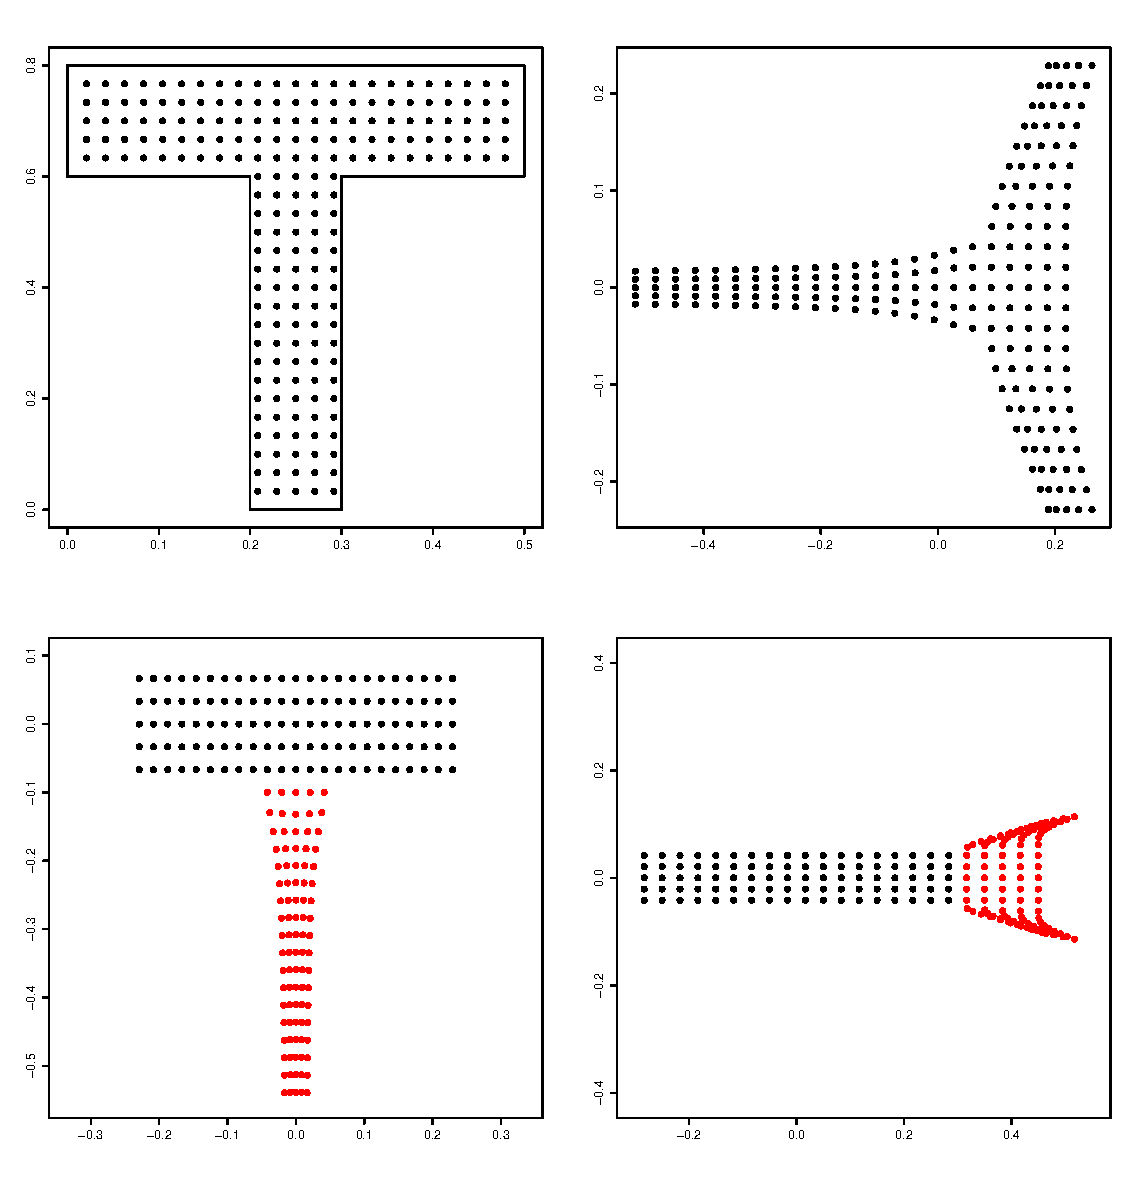
\includegraphics[width=3.5in]{mds/figs/tshape.pdf} \\
\caption{Data generated inside a T-shape (top left) is fed into MDS at once (top right). When either the head or tail of the T is used for the original MDS configuration and the other points inserted, the shape produced is distorted.}
\label{tshape}
% generated using figs/gridtest.R
\end{figure}

Although the cases show in \fig{tshape} are somewhat pathological, looking at more reasonable situations still leads to wildly different results. In \fig{tshaperand} the black and green points make up the original MDS configuration; the five green points are chosen at random. The red points are then inserted. As can be seen in these four typical realisations, the shape of the MDS space is dependent on those points used to create the initial MDS configuration.

% showing the the grid is necessary using the T shape (random samples
\begin{figure}
\centering
% trim order l b r t
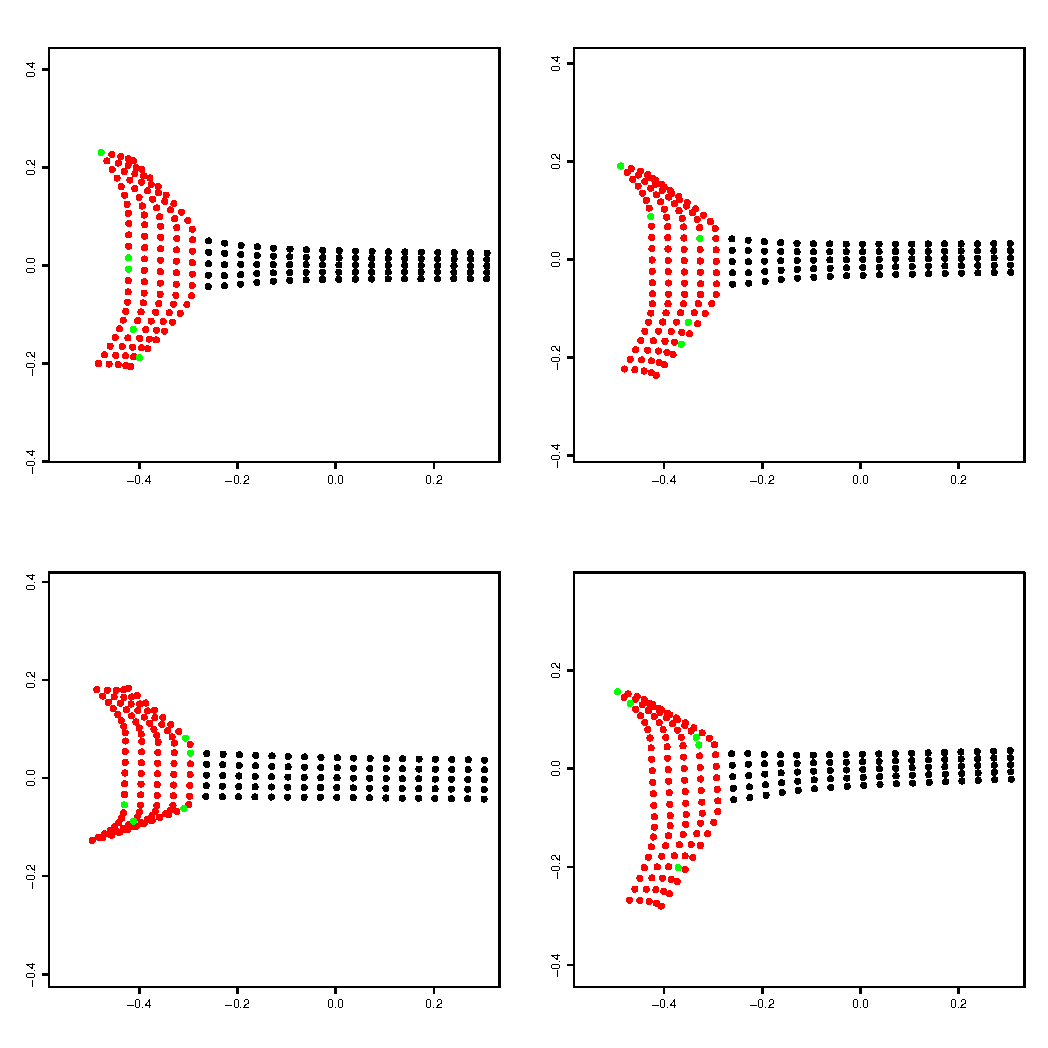
\includegraphics[width=3.5in]{mds/figs/tshaperand.pdf} \\
\caption{Using the T-shape in \fig{tshape} (top left), the tail (black points) of the T was used with 5 randomly sampled (green) points in the head. The head (without the 5 green points) was then inserted into the MDS configuration (red). As can be seen from these four realisations, the output varies greatly depending on the points sampled.}
\label{tshaperand}
% generated using figs/gridtest.R
\end{figure}

Hence, although there are the usual problems with predicting outside of the data, the added problem of the instability of MDS insertion can only confound results further. (Again, this is mentioned at the end of Gower's paper).

This problem can be rectified by using an appropriately spaced grid on the domain to calculate the eigen-decomposition, thus ensuring that the whole domain is covered. The base MDS configuration is then stable, provided that the grid is fine enough to catch all of the important features in the boundary of the domain.

\subsubsection{Smoothness of mapping}
\label{mds-smoothness}

Following from this, it is important to make sure that the MDS space is smooth in the sense that a grid of smooth lines over the domain are mapped to a series of smooth lines without discontinuities or sudden changes in direction. Taking the evenly spaced 50 by 50 point grid in \fig{wt2-grid-orig}, first MDS is performed on a dense point set of size 1253, and then a less dense grid is inserted using the method of Gower. The grid produced under the insertion can be seen in \fig{wt2-grid-full}. Taking a sample of 250 points from the 1253, an MDS configuration was also found and the same grid inserted (see \fig{wt2-grid-samp}). From this it is clear that those points mapped into the domain are smooth but in the sample case the features in the far right of the shape (the less pronounced peninsulae) are slightly squashed.

% grid to map
\begin{figure}
\centering
% trim order l b r t
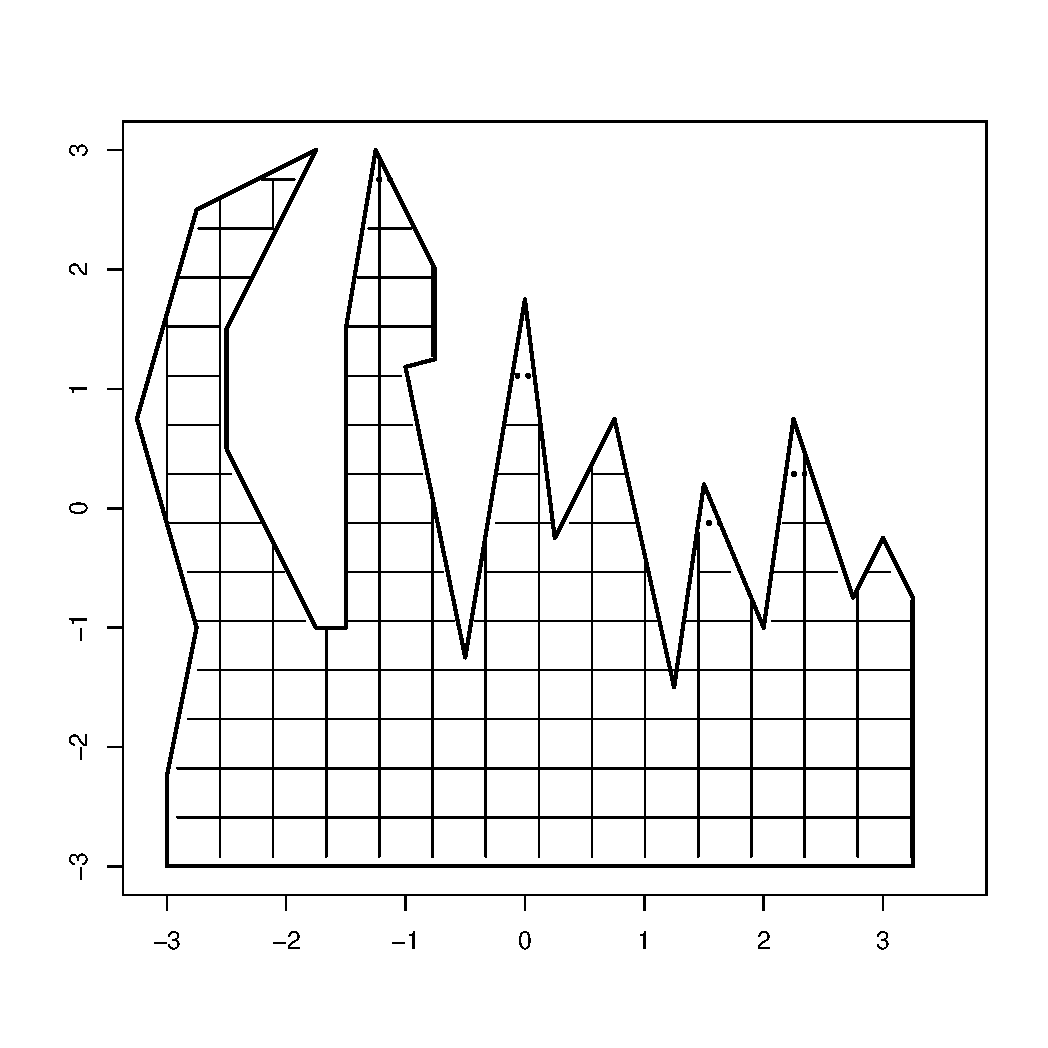
\includegraphics[width=4in]{mds/figs/wt2-grid-orig.pdf} \\
\caption{The grid to be inserted into the MDS configuration over the peninsula domain to test the smoothness of the mapping.}
\label{wt2-grid-orig}
% generated using wt2-grid.R
\end{figure}

% mapped grid (full)
\begin{figure}
\centering
% trim order l b r t
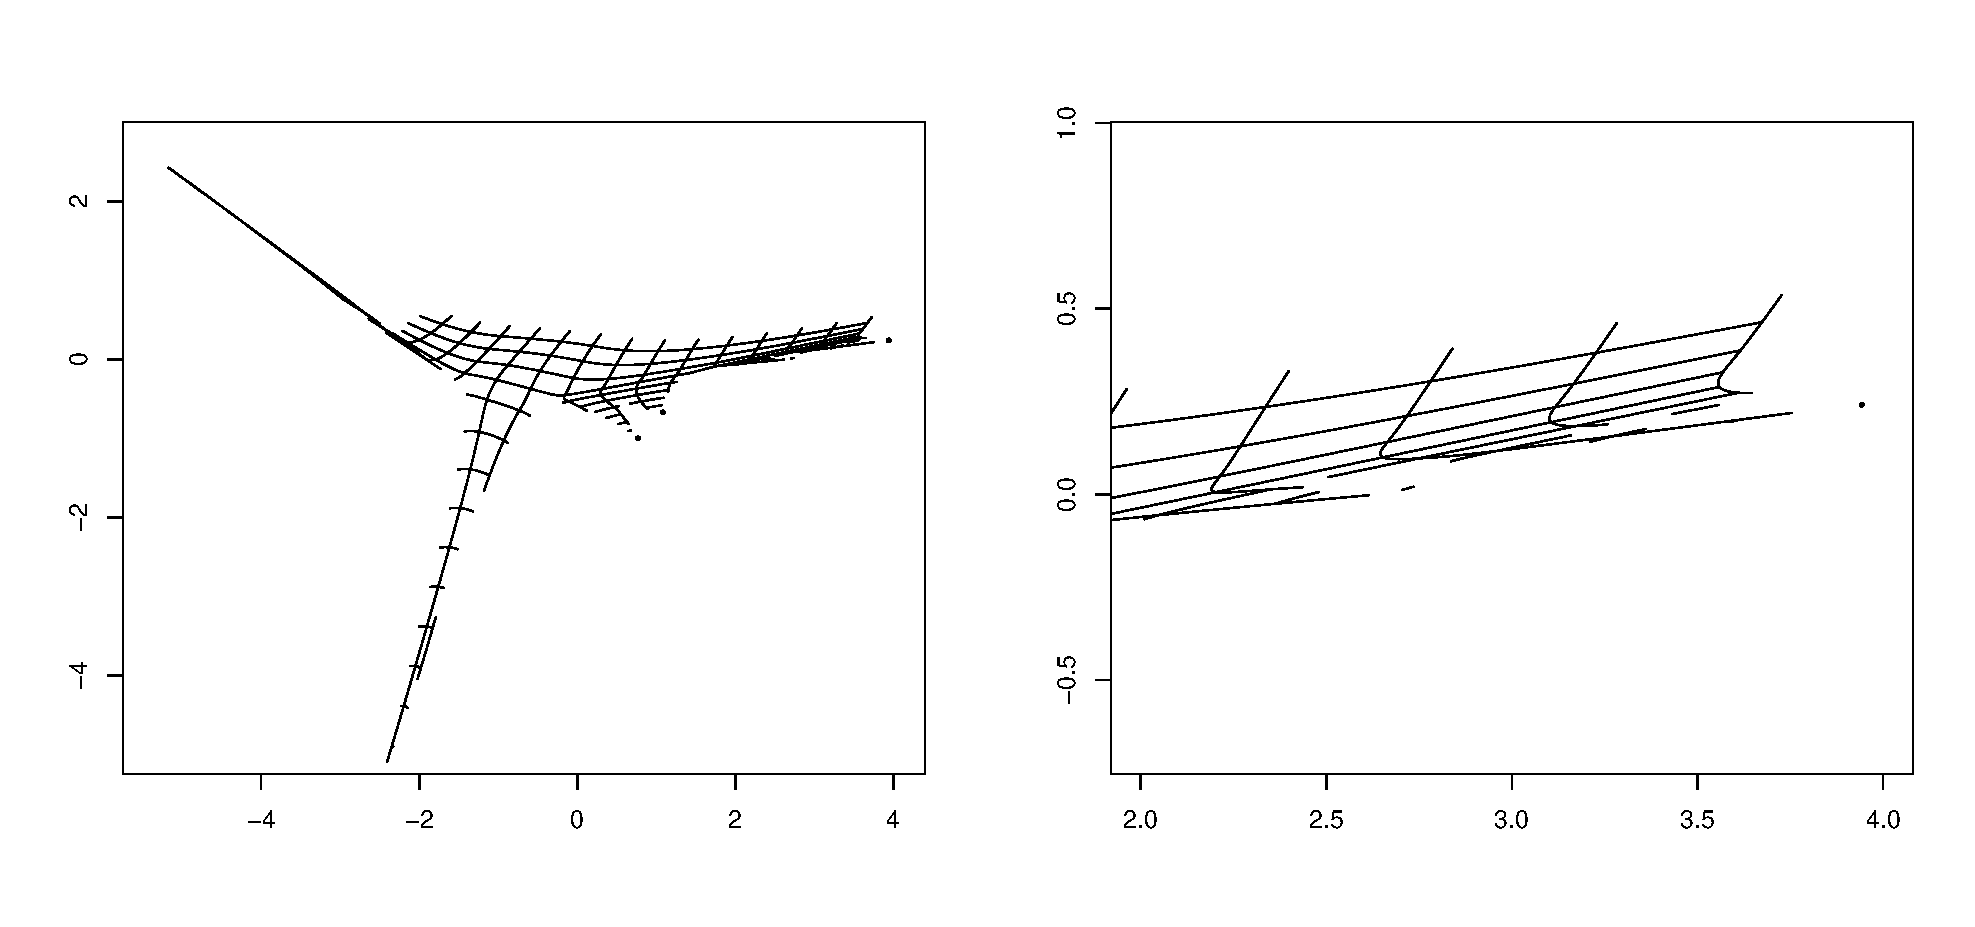
\includegraphics[width=5in]{mds/figs/wt2-grid-full.pdf} \\
\caption{Inserted grid when 1253 points are used to create the initial MDS configuration. The right panel shows a zoom of the far right part of the configuration.}
\label{wt2-grid-full}
% generated using wt2-grid.R
\end{figure}

% mapped grid (samp)
\begin{figure}
\centering
% trim order l b r t
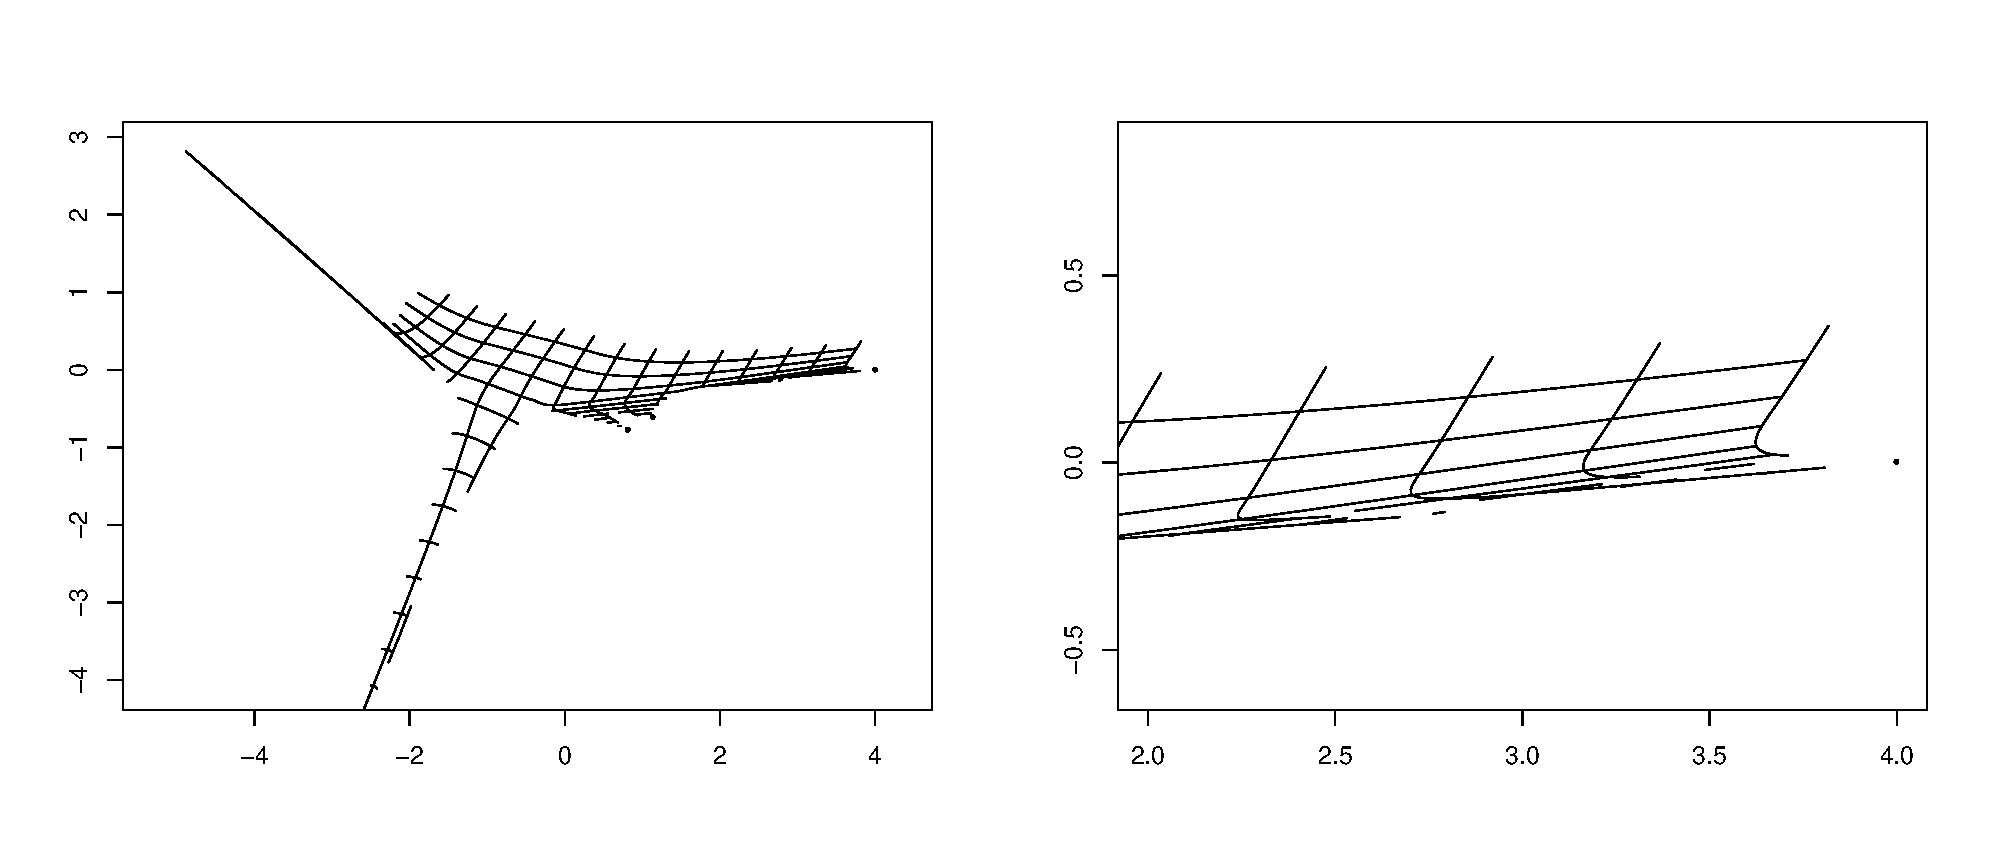
\includegraphics[width=5in]{mds/figs/wt2-grid-samp.pdf} \\
\caption{Inserted grid when 250 randomly chosen points are used to create the initial MDS configuration. The right panel shows a zoom of the far right part of the configuration. Comparing this to that of \fig{wt2-grid-full}, one can see that the features on the right have been squashed together.}
\label{wt2-grid-samp}
% generated using wt2-grid.R
\end{figure}

In conclusion, the mapping can be both reliable and also produces a smooth configuration of points provided that the initial MDS configuration covers the space in sufficient detail.


\section{Finding the within-area distances}
\label{mdsdist}
In order to perform multidimensional scaling the matrix of distances must be found. This section describes a novel algorithm to find the within-area distances.

Let the domain boundary be some polygon, $\Gamma$. Given that there is no direct path within the domain between two points ($p_1$ and $p_2$, say), the algorithm proceeds as follows to create a path (ie. an ordered set of edges and vertices), $\mathcal{P}$:

\begin{enumerate}
\item (INIT) Start by drawing a line between $p_1$ and $p_2$ (\fig{wdia}, ($i$)). Start the path as the lines from $p_1$, $p_2$ to their nearest intersection with the boundary of $\Gamma$ ($p_1^1$, $p_2^1$, say). Then form two paths. The first path from $p_1^1$ to $p_2^1$ ($\mathcal{P}_1$) contains the vertices of $\Gamma$ found moving along the boundary from $p_1^1$ to $p_2^1$. The second ($\mathcal{P}_2$), is found by taking the path from $p_1^1$ to $p_2^1$ in the other direction around the boundary, ie. the vertices of $\Gamma$ not in the first path. It is easy to see that $\{\mathcal{P}_1 \cup \mathcal{P}_2\} \setminus \{p_1^1, p_2^1\} = \Gamma$. The DELETE step (below) is then performed on $\mathcal{P}_1$ and $\mathcal{P}_2$, removing any superfluous vertices. Finding the length of $\mathcal{P}_1$ and $\mathcal{P}_2$ and choosing the shorter ($\mathcal{P^*}$), the initial path is formed as $\mathcal{P}=(p_1,p_1^1,\mathcal{P}^*,p_2^1,p_2)$. 

In \fig{wdia}, ($iii$), $\mathcal{P}_1$ is marked in green and is chosen to form the initial path, $\mathcal{P}=(p_1,p_1^1,\mathcal{P}_1,p_2^1,p_2)$, as $\mathcal{P}_1$ is shorter than $\mathcal{P}_2$, in red.

\item (DELETE) Given a triple of vertices, $(v_i, v_{i+1}, v_{i+2}) \in \mathcal{P}$ , if the line between $v_i$ and $v_{i+2}$ is shorter than the path $(v_i, v_{i+1}, v_{i+2})$ and the line between $v_i$ and $v_{i+2}$ lies inside $\Gamma$ then delete $v_{i+1}$ (\fig{wdia}, ($iv$) and ($vi$)). The entire path is iterated over deleting all superfluous vertices until there are no changes in successive runs. 

For example in \fig{wdia} ($iii$), $v_2$ is deleted from $\mathcal{P}$ because the path straight between $v_1$ and $v_3$ is shorter, and within $\Gamma$.

\item (ALTER) Given a triple of vertices $(v_i, v_{i+1}, v_{i+2}) \in \mathcal{P}$, if the path $\mathcal{P}_{ID}$ is shorter than the path $(v_i, v_{i+1}, v_{i+2})$ then replace $(v_i, v_{i+1}, v_{i+2})$ with $\mathcal{P}_{ID}$ (\fig{wdia}, ($v$)). The candidate replacement path, $\mathcal{P}_{ID}$, is calculated by running INIT with $p_1$ and $p_2$ replaced by $v_i$ and $v_{i+2}$, producing $\mathcal{P}_I$, and then using DELETE on $\mathcal{P}_I$ to remove superfluous vertices, giving $\mathcal{P}_{ID}$.

For example in \fig{wdia} ($iv$), the path $(v_1, v_2, v_3)$ is longer than the path $\mathcal{P}_{ID}=(v_1, v^1_2, v_3)$ (green dashed line in ($iv$)) so the former is replaced with the latter in $\mathcal{P}$. The path created by INIT is marked as $\mathcal{P}_{I}$ in  ($iv$) in red.

\item (ITER) We then iterate further DELETE and ALTER steps until there has been no change in $\mathcal{P}$ from one run to the next (ie. convergence) (\fig{wdia}, ($vi$)).
\end{enumerate}

% diagram for finding the shortest path in W
\begin{sidewaysfigure}
\centering
% trim order l b r t
\psfrag{exp1}[]{$\mathcal{P}_1$}
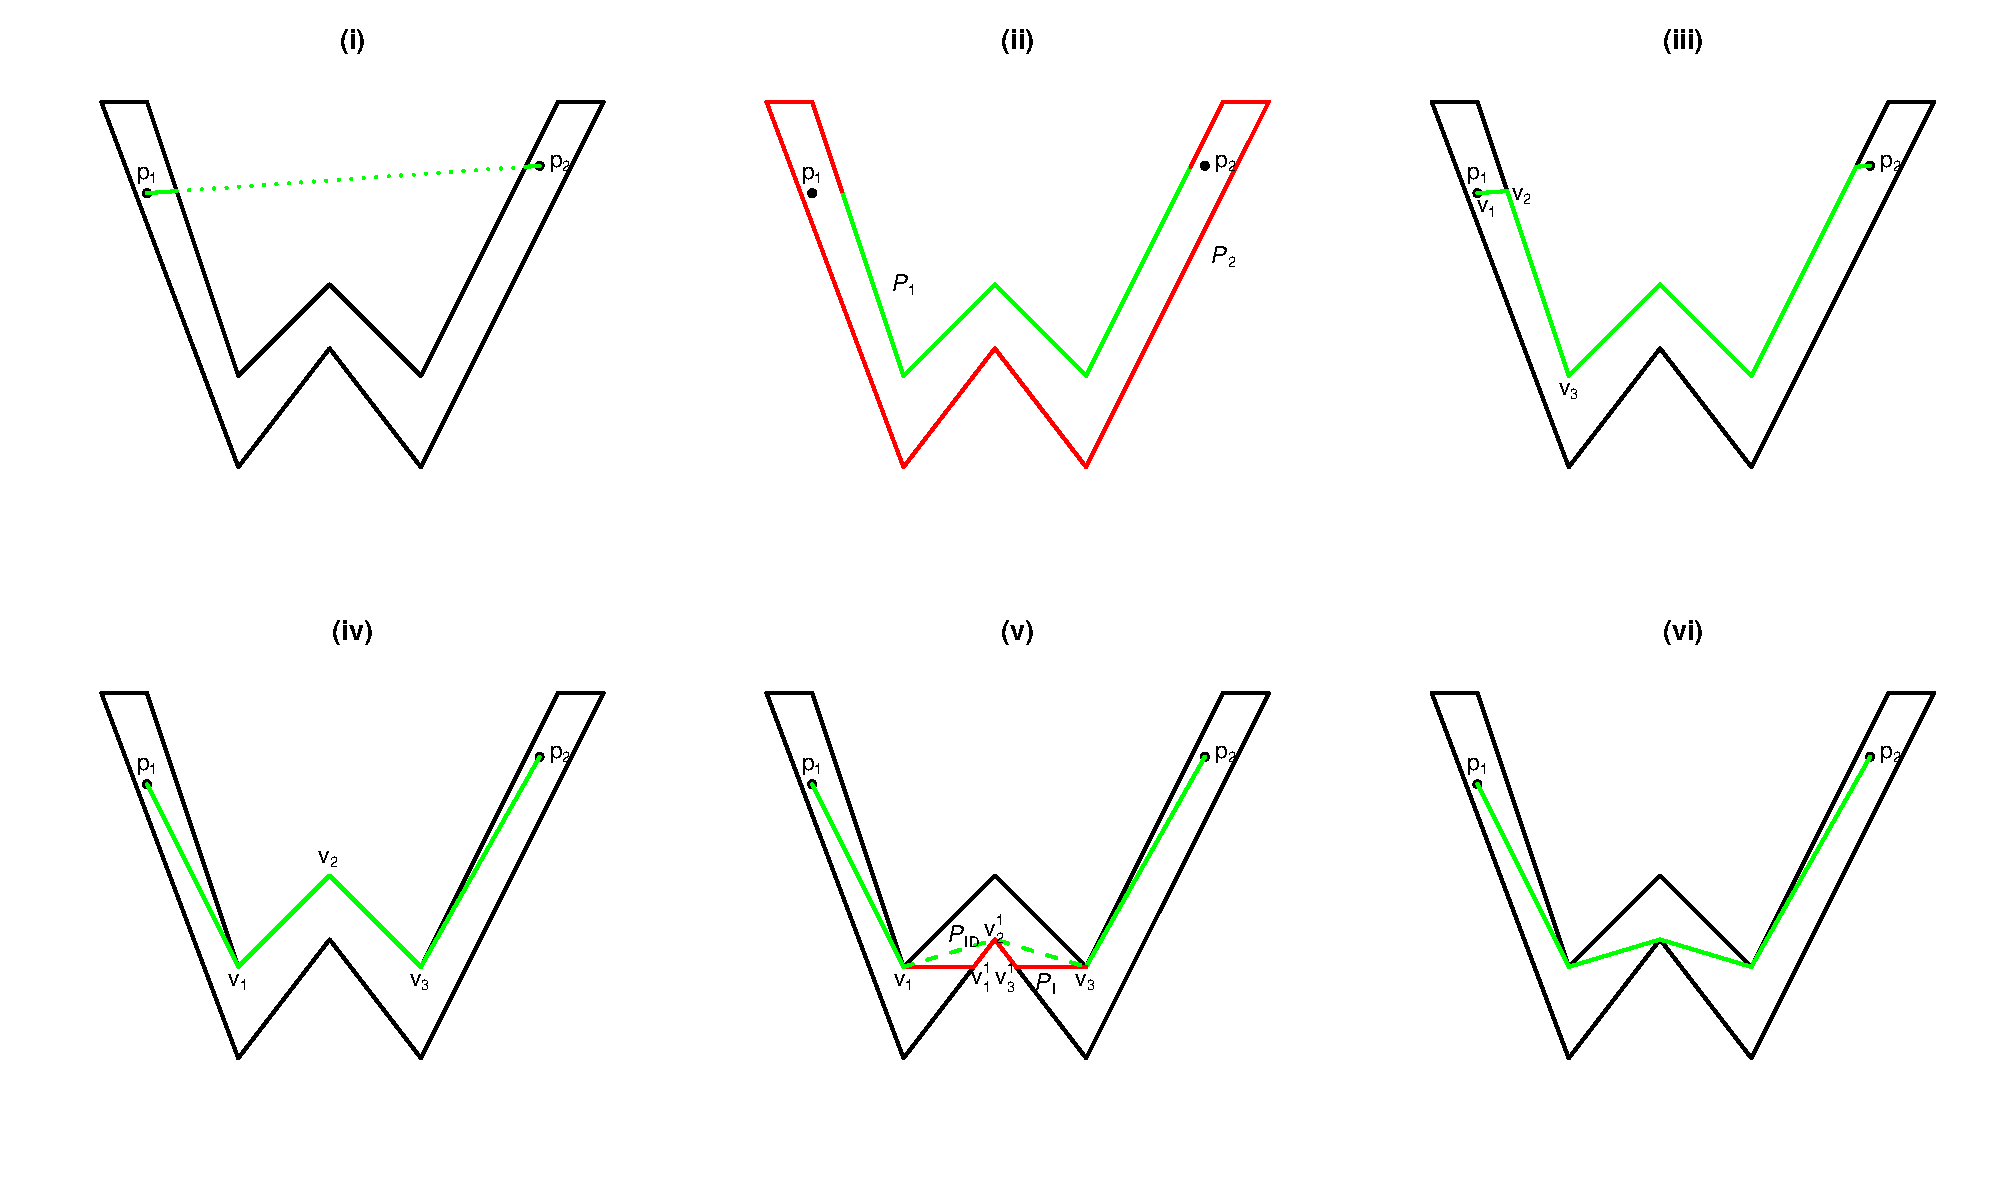
\includegraphics[trim=0in 0.5in 0in 0.25in, width=9.5in]{mds/figs/wdia.pdf} \\
\caption{The green lines in ($i$) to ($vi$) show the steps forming the shortest path as the algorithm progresses from initial state to final, shortest path (bottom right). See \secref{mdsdist}.}
\label{wdia}
% generate /phd-smoothing/mds-writeup/figs/distanceexplanation.R
\end{sidewaysfigure}

Of course, if there is a direct path between $p_1$ and $p_2$ then the Euclidean distance between the points can be used.

\section{Simulation experiments}
\label{mdssims}

In order to investigate the efficacy of \mdsap, a series of simulation experiments were performed. In all cases the results for \mdsap\ were compared to those of the current best method (the soap film smoother) and the standard approach of a {\tprs\} was used (which will not account for leakage).

The \textsf{R} packages \texttt{mgcv} and \texttt{soap} with additional bespoke software for finding the within-area distances were used. In all cases smoothing parameter estimation was performed using GCV (see \secref{GAMGCV}).

\subsection{The Ramsay horseshoe}

Again, we start with the modified Ramsay horseshoe since it clearly illustrates the problem of leakage; if a general method is to be useful it must first perform well on even a simple case such as this.

\subsubsection{Setup}

For the horseshoe, samples of 250 points with normal errors (at 3 levels:  $\sigma= $ 0.1, 1 and 10) were taken. (These are the settings used in \cite{soap}.) Using these samples, three models were fitted to the data. Predictions were then made over 718 points (including the sample locations). 200 realisations were generated and the EDF and MSE recorded for each replicate. The three models fitted were as follows:

\begin{enumerate}
\item \emph{Thin plate spline}: bivariate \tprs\  with basis size 100.
\item \emph{Soap film smoother}: 32 knots evenly spread over a grid over the domain, cyclic spline on the boundary was of basis size 39.
\item \emph{\mdsap}: Used a thin plate spline of basis dimension 100. The initial MDS grid was 20 points wide by 10 points tall.
\end{enumerate} 

Note that due to time and computational restrictions, the boundary was reduced from the 160 vertex polygon in the \texttt{fs.boundary()} function in \texttt{soap} to a 21 vertex polygon by only using every 8$^\text{th}$ vertex. This should not cause a major difference in results even if the soap film used the full boundary and \mdsap\ used only the reduced set of edges, since objective is to allow the smoother to get a broad idea of the topology of the domain, rather than the minutiae of the boundary features.

\subsubsection{Results}

Predictions from a typical realisation can be seen from \fig{mds-ramsay-fit-1}, where $\sigma=1$ with a sample size of 250. Both the soap film smoother and \mdsap\ are able to reproduce the main features of the true horseshoe function due to their ability to respect the boundary (in the case of the soap film) or the geometry of the domain (in the case of \mdsap). The \tprs\ shows leakage as expected. This is reflected in table \ref{ramsayresultstable} where we see that the soap film smoother and \mdsap\ have significantly smaller average MSE. When the noise level is high the \mdsap\ outperforms the soap film smoother in MSE terms (and is less variable).

\begin{table}[ht]
\centering
\begin{tabular}{c c c c}
 & & MSE & \\ 
$\sigma$ & \mdsap & Soap film & Thin plate\\ 
\hline
0.1  & 0.0032 (3$\cross10^{-5}$) & 0.0022 (3$\cross10^{-5}$) & 0.0402 (0.0008) \\ 
1  & 0.0436 (0.0015) & 0.0482 (0.0014) & 0.2306 (0.0024) \\ 
10  & 2.0652 (0.1215) & 3.0702 (0.2382) & 3.3713 (0.1133) \\ 
\end{tabular}
\begin{tabular}{c  c c c }
&  & EDF & \\ 
$\sigma$ & \mdsap & Soap film & Thin plate\\ 
\hline
0.1 & 47.613 (0.3497) & 39.164 (0.26) & 92.5996 (0.1020)\\ 
1  & 8.3828 (0.3452) & 11.868 (0.4010) & 46.607 (0.4238)\\ 
10 & 5.0577 (0.3324) & 5.5863 (0.2876) & 5.9786 (0.2511)\\ 
\end{tabular}
\caption{Mean MSE and estimated degrees of freedom (EDF) for the three models fitted to the modified Ramsay horseshoe function with standard errors (in brackets) over 200 realisations. Sample size was 250 with error levels given in the column marked $\sigma$.}
\label{ramsayresultstable}
\end{table}

The EDFs in table \ref{ramsayresultstable} show that \mdsap\ fits a less complex model than the thin plate spline on average, and for the two higher error situations, has a lower EDF than the soap film. Given that this is coupled with a lower MSE, it appears that \mdsap\ simultaneously yields both a more accurate and less complex model than the soap film for the horseshoe when there is a high level of noise. When noise is lower, the soap film and \mdsap\ MSEs are still of the same order. \Fig{mds-ramsay-boxplot} shows the logarithm of the per-realisation average MSE for each of the models at each error level.

% boxplot for Ramsay
\begin{figure}
\centering
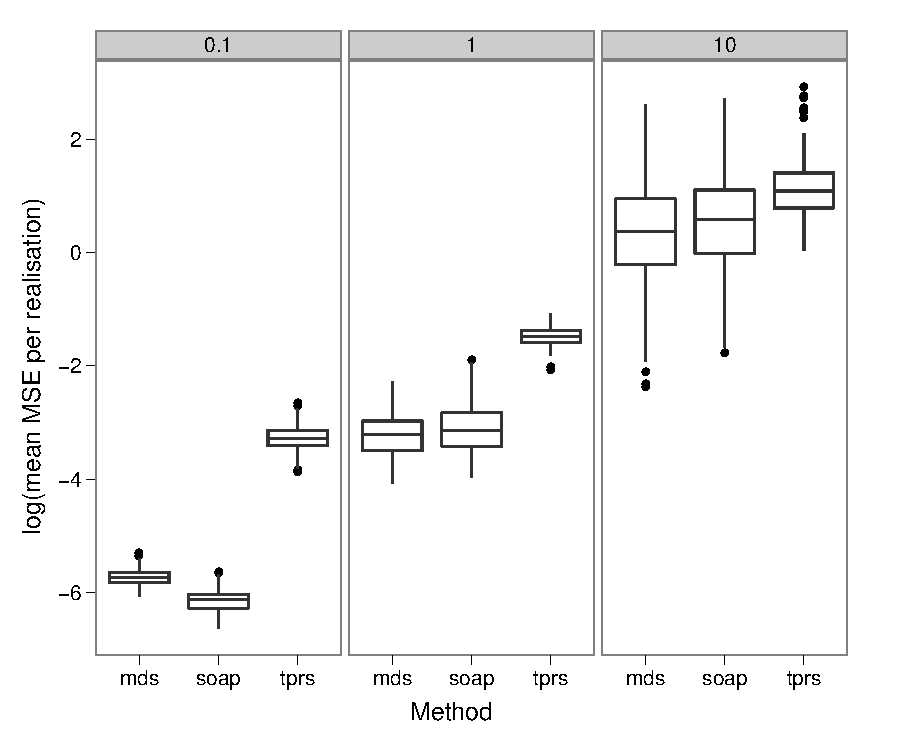
\includegraphics[width=6in, trim=0in 0.5in 0in 0in]{mds/figs/mds-ramsay-boxplot.pdf} \\
\caption{Boxplots of the logarithm of the MSE per realisation of the Ramsay horseshoe for \mdsap\, the soap film smoother and \tprs\ for error levels $\sigma=$ 0.1, 1 and 10 (left to right, respectively). In all cases, a Wilcoxon signed rank test showed that MSEs for \mdsap\ and \tprs\ were significantly different from the soap film smoother ($\text{p-value} < 10^{-2}$).}
\label{mds-ramsay-boxplot}
% generated using phd-smoothing/mds/sim/ramsay-boxplots.R
% Wilcoxon test in phd-smoothing/mds/sim/ramsay-wilcox.R
\end{figure}

% Ramsay fit with error=1 
\begin{figure}
\centering
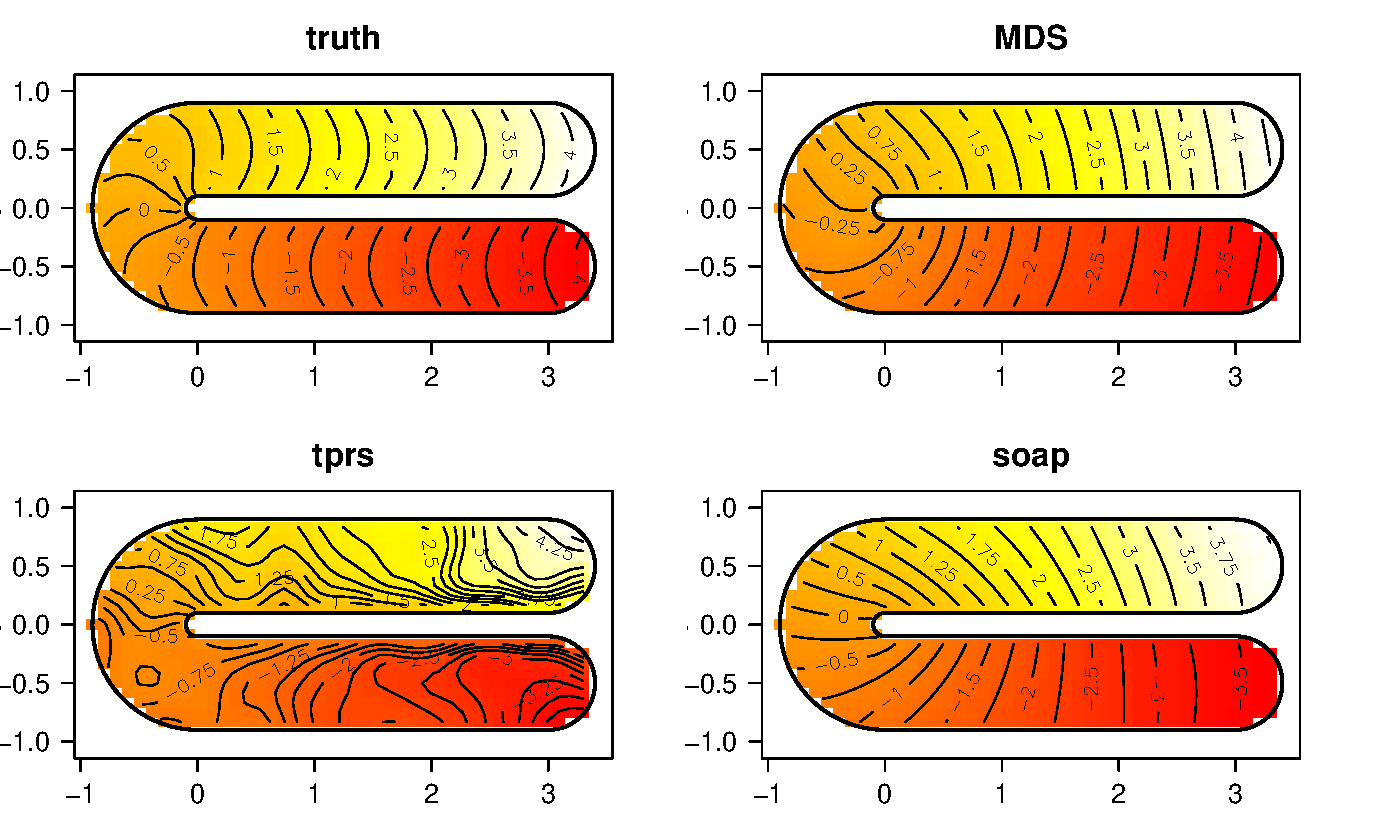
\includegraphics[width=6in]{mds/figs/ramsay-fit-1.pdf} \\
\caption{Top left: truth for the (modified) Ramsay horseshoe. Others: a typical realisation of fits from the three models when 250 points are sampled with noise set to $\sigma=1$.}
\label{mds-ramsay-fit-1}
% generated (roughly) using ramsay-smooth-test.R
\end{figure}

Just as when the \sch\ transform was used to morph the domain, it is interesting to see what has happened to the distribution of points in space. \Fig{mdsrampoints} shows the effect of the transform on a regular grid of points (left) when they are projected into MDS space (right). The projection has also succeeded in parting the two arms of the horseshoe, reducing leakage (as can be seen in the realisations in \fig{mds-ramsay-fit-1}).

\begin{figure}
\centering
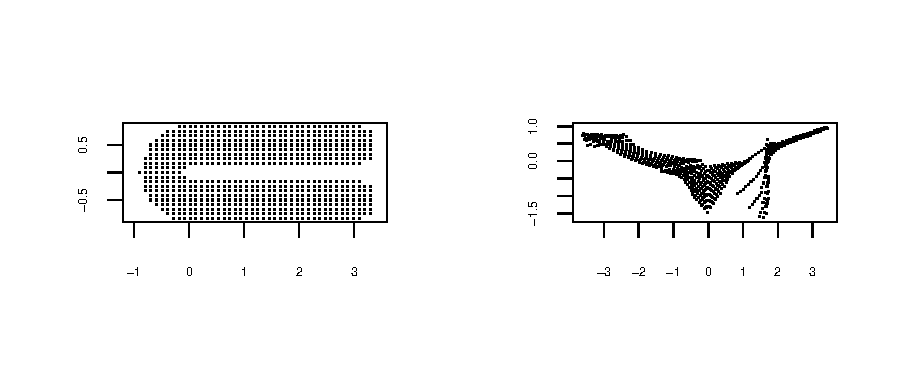
\includegraphics[width=6in,trim=0.5in 0.5in 0in 0.5in]{mds/figs/mdsrampoints.pdf} \\
\caption{A regular grid over the Ramsay horseshoe (left) and its projection into MDS space (right).}
\label{mdsrampoints}
% generated using thesis/mds/figs/mdsrampoints
\end{figure}


\subsection{Peninsula domain}
\label{mds-wt2-sim}

The Ramsay horseshoe is an easy domain to smooth over since it is clear that a transformation should be parting the two arms of the domain. In practise however, there may be ambiguity over which parts of the domain should be separated the most. For this reason a more realistic, complex domain would provide a better insight into the efficacy of the method. The domain shown in \fig{wt2-truth} is an approximation to a coastline with a strong trend along both peninsulae (in a manner similar to that of the horseshoe) but with the added complication of a further peak in the lower right corner.

\subsubsection{Setup}

The simulations consisted of 200 realisations of 250 samples from the surface in \fig{wt2-truth}. Normal errors were added at three levels $\sigma=$ 0.35, 0.9, and 1.55 (corresponding to signal-to-noise ratios (SNRs) of 0.95, 0.75 and 0.5, respectively. SNRs were calculated as the mean squared correlation between true function value and the truth with error added). Mean squared error over 1253 prediction points (including those points in the sample) was calculated and recorded, along with EDF for each model. The models fitted were:

% wt2 truth 
\begin{figure}
\centering
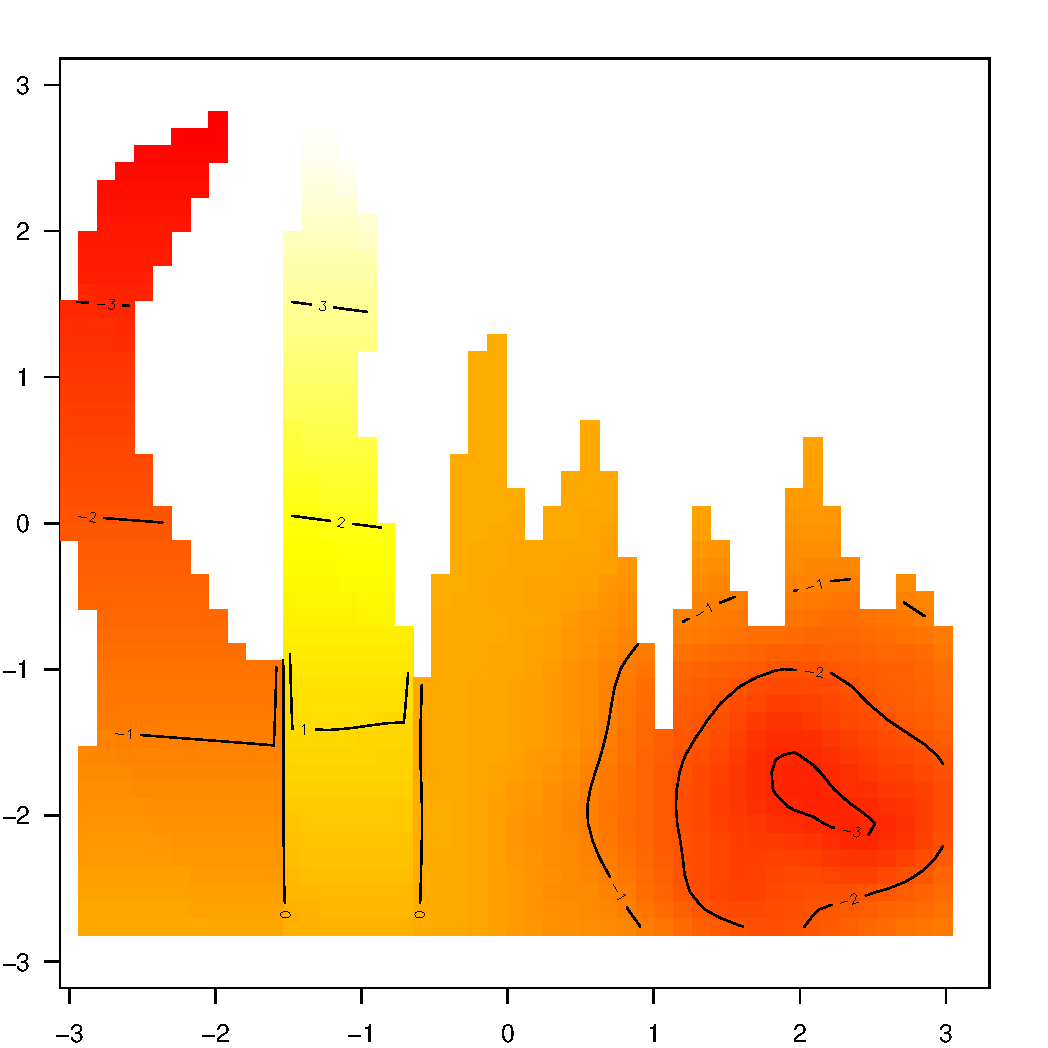
\includegraphics[width=3in]{mds/figs/wt2-truth.pdf} \\
\caption{True function for the domain with multiple peninsulae.}
\label{wt2-truth}
% generated (roughly) using wt2-smooth-test.R
\end{figure}

\begin{enumerate}
\item \emph{Thin plate spline}: bivariate thin plate spline with basis size 100. 
\item \emph{Soap film smoother}: cyclic spline on boundary of basis size 60, 109 internal knots evenly spaced on a grid over the domain.
\item \emph{\mdsap}: after transform a bivariate thin plate spline with basis size 100 was fit. The initial MDS grid was 10 by 10 points square (48 points were inside).
%\item \emph{MDS with tensor product}: tensor product of two thin plate splines, each of basis dimension 12. The initial MDS grid was 74 points square.
\end{enumerate} 

\subsubsection{Results}

% wt2 fit with error=0.9
\begin{figure}
\centering
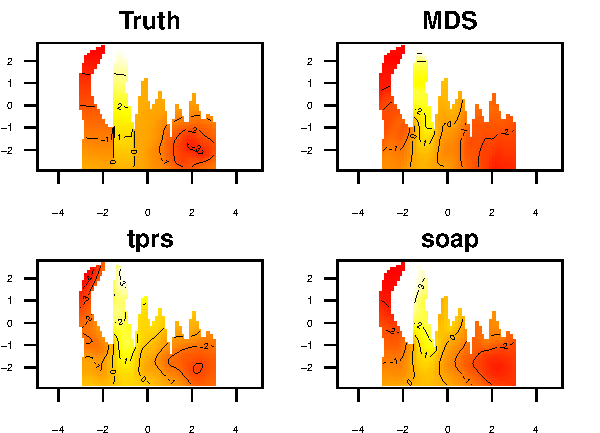
\includegraphics[width=6in]{mds/figs/wt2-comp-09.pdf} \\
\caption{A typical realisation of fits from the multiple peninsulae domain when $\sigma$ is set to 0.9 (SNR = 0.75) and sample size is 250. Prediction grid was of size 1253. Clockwise from top left: the true function, prediction from: MDS projection smoothed with \tprs, the soap film smoother and \tprs.}
\label{wt2-comp-0.9}
% generated (roughly) using wt2-smooth-test.R
\end{figure}

Looking at a typical realisation in \fig{wt2-comp-0.9} ($\sigma=$ 0.9, SNR = 0.75, sample size 250), the \tprs\ can be seen showing signs on leakage across the two main peninsulae, whereas \mdsap\ and the soap film do not show this. However the \tprs\ does reproduce the peak in the lower right much more faithfully, the other two smoothing over it. In this realisation, \mdsap\ deals with the values inside the peninsula a little better than the soap film smoother (the contour lines are closer to those in the true function). On the other hand, the soap film captures the shape of the lower right peak slightly more accurately.

Table \ref{wt2resultstable} gives the MSE and EDF for the models above averaged over 200 realisations. There is not a massive difference between the results in MSE terms, the soap film smoother consistently has a lower MSE, although not by much. The soap film also tends to fit simpler models than the other two approaches. The boxplots of the logarithm of the per-realisation MSEs are shown in \fig{mds-wt2-boxplot}.

% boxplot for wt2
\begin{figure}
\centering
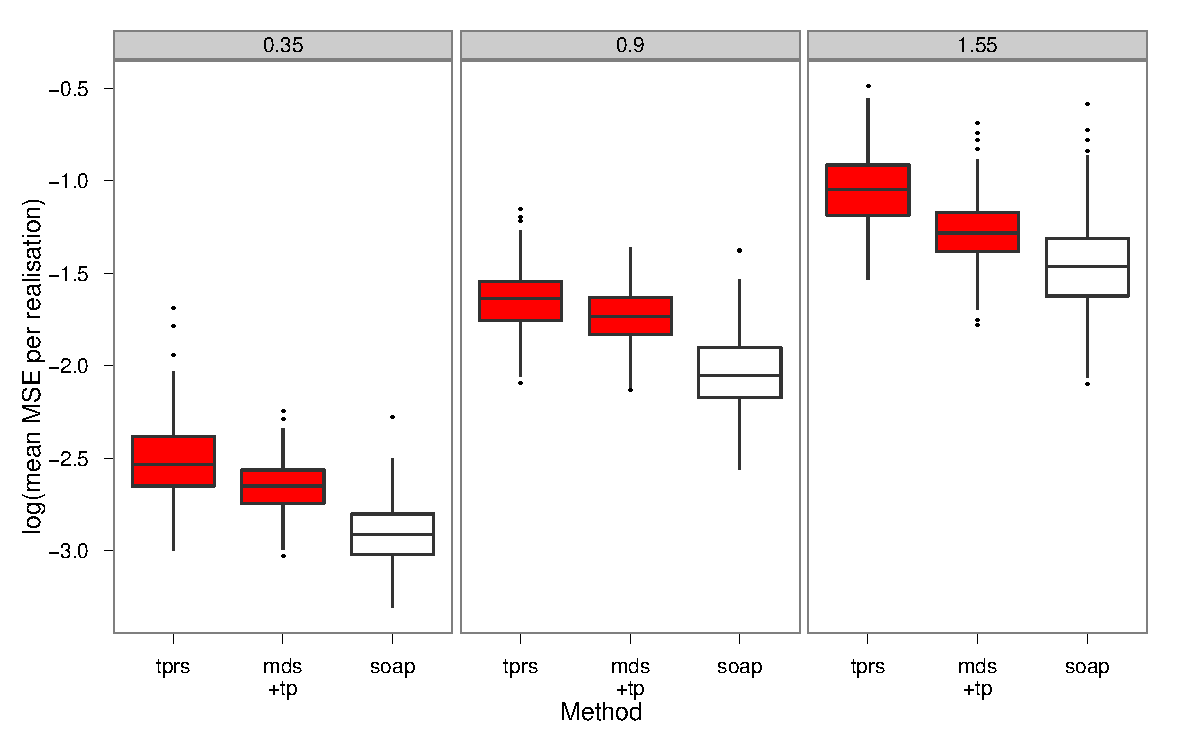
\includegraphics[width=6in, trim=0in 0.5in 0in 0in]{mds/figs/mds-wt2-boxplot.pdf} \\
\caption{Boxplots of the logarithm of the MSE per realisation of the peninsula domain for the MDS approach, soap film smoother and \tprs\ for error levels $\sigma=$ 0.35, 0.9 and 1.55 (left to right, respectively). A Wilcoxon signed rank test shows that the MSEs for \tprs\ were significantly different from those of the soap film smoother ($\text{p-value} < 10^{-2}$) at all noise levels. For \mdsap\ the two lower noise cases were significantly different from the soap film smoother, but not when $\sigma=1.55$ ($\text{p-value} = 0.023951$).}
\label{mds-wt2-boxplot}
% generated using phd-smoothing/mds/sim/wt2-boxplots.R
\end{figure}

\begin{table}[ht]
\centering
\begin{tabular}{c c c c c}
 &  & MSE  & &\\ 
$\sigma$ & \mdsap & Soap film & Thin plate\\ 
\hline
0.35  & 0.07 (0.00062) & 0.0539 (5e-04) &0.082 (0.00104)\\
0.9  & 0.177 (0.00184) & 0.1308 (0.00197) &0.1938 (0.00241)\\
1.55  & 0.2859 (0.00438) & 0.2362 (0.00434) &0.3509 (0.00471)\\
\end{tabular}
\begin{tabular}{c c c c c}
 &  & EDF  & &\\ 
$\sigma$ & \mdsap & Soap film & Thin plate\\ 
\hline
0.35 &80.9039 (0.57103) & 55.6979 (0.51448) & 77.9619 (0.46726)\\ 
0.9 &35.0185 (0.76449) & 29.7171 (0.57477) & 48.0508 (0.47636)\\ 
1.55 &19.4625 (0.57265) & 20.2918 (0.36634) & 32.2715 (0.47961)\\ 
\end{tabular}
\caption{Mean MSE and EDF for the three models fitted to the peninsula domain with standard errors (in brackets) over 200 realisations.}
\label{wt2resultstable}
\end{table}

As with the Ramsay horseshoe, it is interesting to see what the projection into MDS space has done to the distribution of the points in the domain. \Fig{wt2-2d-proj} shows points in the domain in Euclidean space and MDS space. There appears to be some high concentrations of points in the far left peninsula and in the right side in the MDS space. This is due to the projection from $n$-dimensional space into 2-dimensional space, which can be easily seen in \fig{wt2-3d-proj} where the points have been projected into 3-dimensional space. This shows that there is separation between the smaller peninsulae in higher dimensions that cannot be seen in the 2-dimensional projection.

This high point density in the right side of the MDS space could be the reason for the poor reproduction of the function in that region, seen in \fig{wt2-comp-0.9}. In this portion of space (and in the left peninsula) there is a breakdown in isotropy, which the \tprs\ does not handle well. This must be accounted for in the smooth if accurate models are to be built.

% how the points are projected for wt2
\begin{figure}
\centering
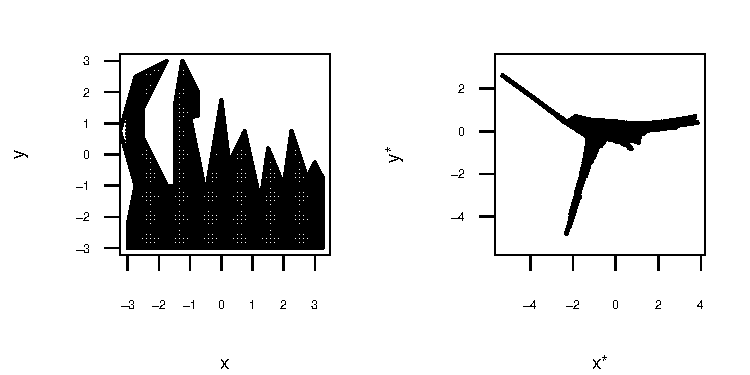
\includegraphics[width=6in]{mds/figs/wt2-2d-proj.pdf} \\
\caption{A regular grid over the peninulae domain (left) and its projection into MDS space (right).}
\label{wt2-2d-proj}
% generated using thesis/mds/figs/wt2-mds.R
\end{figure}

% how the points are projected for wt2 in 3D!
\begin{sidewaysfigure}
\centering
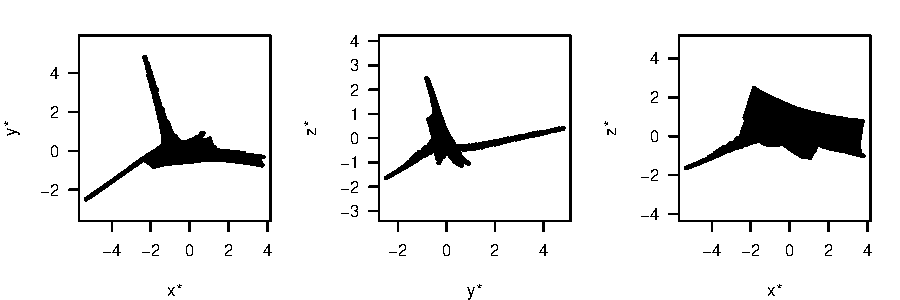
\includegraphics[width=9in]{mds/figs/wt2-3d-proj.pdf} \\
\caption{The peninsula domain projected into 3-dimensional MDS space. The plots show combinations of axes, note that the $x^*,y^*$ combination is the same as the 2-dimensional projection in \fig{wt2-2d-proj}.}
\label{wt2-3d-proj}
% generated using thesis/mds/figs/wt2-mds.R
\end{sidewaysfigure}

\subsection{Areas for improvement}

From this set of simulations areas for improvement to \mdsap\ can be seen. First, the above problem of the accuracy of the model (in terms of faithfully reproducing the function) needs to be addressed. Second, running the model is actually quite slow, the calculation of the within-area distances by the algorithm given in \secref{mdsdist} has considerable computational cost, even in comparison to the soap film smoother basis setup. Table \ref{wt2time} shows the average timings for running \mdsap, \tprs\ and soap film smoothers over the peninsula domain

\begin{table}[ht]
\centering
\begin{tabular}{c || c c c c c c}
 & \mdsap & Soap film & Thin plate\\ 
\hline
Fit & 84.85242 & 24.6783 & 0.4022\\ 
Prediction &  53.5105 & 29.3946 & 0.1249\\
\end{tabular}
\label{wt2time}
\caption{Average time (in seconds) to fit and predict on a realisation of the peninsula domain for the three models considered above. Times are averaged over 100 realisations and were found using the elapsed time provided by \textsf{R}'s built-in \texttt{system.time} function. For each realisation a sample of size 250 was taken, then a 1253 values were predicted.}
\end{table}

In order to make \mdsap\ worthwhile for a practitioner to use the method, it would be preferable for it not only to have a sensible physical model, but also outperform the soap film smoother in either (or both) of accuracy and speed.

\section{Making \mdsap\ faster}
\label{mds-faster}

\subsubsection{Calculating MDS by Lanczos iteration}

The \textsf{R} command used to perform the multidimensional scaling, \texttt{cmdscale}, uses the routine \texttt{eigen} in order to perform the requisite matrix eigen-decomposition. This routine will calculate a full eigen-decomposition of the matrix, even if only the first $k$ eigenvalues and/or eigenvectors are required. Using Lanczos iteration, only the first $k$ eigenvalues (in numeric or algebraic size order) will be calculated.

The  Lanczos procedure works by iteratively building a symmetric $i\cross i$ tridiagonal matrix (at the $i^{\text{th}}$ iteration) which has eigenvalues approximately the same as the $i$ largest eigenvalues of the original matrix. Further detail is given in \cite{simonbook}, pp. 335-337.

The \texttt{igraph} library for \textsf{R} provides an interface to the C++ package \texttt{ARPACK++} which implements the Lanczos procedure. Replacing the \texttt{cmdscale} command with one that uses the \texttt{ARPACK++} interface provided by \texttt{igraph} will decrease the number of computations needed, thus making the calculation of the eigenvalues and vectors faster.

A quick benchmark shows that \texttt{ARPACK++} can compute the first two eigenvalues and vectors faster than just using \texttt{eigen} when the eigen-decomposition to be computed is of a large matrix. Generating a 1000 by 1000 symmetric matrix of Normal random variates with mean 0 and variance 1000, then performing an eigen-decomposition takes 1.68 seconds using \texttt{ARPACK++} and 3.26 seconds using \texttt{eigen} (averaged over 100 runs). This advantage drops once the matrix is around 100 by 100 and the cost of calling the C++ code begins to dominate; in this case \texttt{ARPACK++} takes 0.037 seconds and \texttt{eigen} takes 0.034 (over 100 runs). Given that the disadvantage is in the order of hundredths of a second and the advantage is a two-fold decrease in computational time, it makes sense to use the \texttt{ARPACK++} code in all cases.

% sim code is at ~/phd-smoothing/mds/lanczos/time-arpack.R

\subsubsection{Partial path calculation}

Many of the distances stored in $D$ are calculated by simply using the Euclidean metric since for the corresponding point pairs, there is no part of the path between them that lies outside of the domain. It is often the case that the paths that need to be calculated are on a grid (for example, when doing prediction). This leads us to believe that there are many sets of paths that are rather similar. These paths may perhaps only differ in their final vertex. Given that, in this case, there is a lot of wasted computational time spent calculating similar paths, it would be useful to exploit this problem, and use it to increase the speed of the path calculation.

The idea here is to use a sparse grid to first calculate a set of paths that are then saved. These saved paths are then form the base of the other paths that need to be calculated. Finally, these paths are optimised in the same manner as the algorithm given in \secref{mdsdist}. This removes the expensive calculation in the middle of the path, where perhaps the bulk of the interactions with the boundary take place.

The algorithm is as follows, with notation and routines (INIT, DELETE, ALTER and ITER) identical to those in \secref{mdsdist}. 

Again, taking points $p_i$ and $p_j$ in the set of points in the domain that we wish to find the shortest paths for and drawing a path between them, finding within-area distance with respect to the boundary of $\Gamma$.

\begin{enumerate}
 \item Begin by creating a sparse grid of within $\Gamma$ and calculate the ($M$, say) non-Euclidean within-area paths between all pairs of points exactly as in \secref{mdsdist}. Store these paths as $\mathcal{P}_1,\ldots, \mathcal{P}_M$.
\item For each unique pairing of $p_i$ and $p_j$ in the full data set, calculate the path using one of the following:
	\begin{enumerate}
	\item Find a $\mathcal{P}_k$ such that the path between $p_i$ and one end of $\mathcal{P}_k$ and $p_j$ and the other end of $\mathcal{P}_k$ is Euclidean within $\Gamma$. Join $p_i$ and $p_j$ onto the appropriate ends of $\mathcal{P}_k$ and run ITER (ie. alternate between DELETE and ALTER) until convergence.
	\item If there is no Euclidean path between $p_i$ and $p_j$, and no $\mathcal{P}_k$ can be found, then calculate the path between $p_i$ and $p_j$ as in \secref{mdsdist}. 
	\end{enumerate}
\end{enumerate}

Note that those paths between points in the sparse grid which are Euclidean are not stored since it is always at least as expensive to store, add and optimise those paths then calculating them from scratch. An argument towards why is this is true is as follows: if the path we want to calculate is Euclidean anyway, then retrieving a Euclidean path, adding in $p_i$ and $p_j$, and then iterating over ALTER and DELETE steps to make it both the shortest and a Euclidean path will take longer than just creating a Euclidean path to begin with. If the path between $p_i$ and $p_j$ is non-Euclidean then the non-Euclidean part of the path must lie outside $\mathcal{P}_k$ (by definition) and therefore will take the same number of operations to find the boundary crossing points and calculate the shortest path around the feature locally as it will to calculating the whole path from scratch.


\subsubsection{Simulation - Lanczos and partial path calculation improvements}

Taking both the Lanczos procedure and the partial path calculation together, a simulation was run to find the improvements in terms of computational time for the double peninsulae domain. Average time for both model fitting and prediction are given in \tabref{wt2itime} for 100 realisations. 

The differences between the first two columns are striking. The partial path calculation has dramatically reduced the computational time for the calculation of the entries of the distance matrix, making it faster than the soap film smoother for the model fitting, and reducing the prediction time to a third of its previous value. The \tprs\ times are shown to give a comparison for the time actually taken to fit the model, the remaining time for \mdsap\ is taken up by calculating the distances and performing the MDS.

\begin{table}[ht]
\centering
\begin{tabular}{c || c c c c c c}
%  no speedup           speedup
 & \mdsap & \mdsap (\textit{pp}) & Soap film & Thin plate\\ 
\hline
Fit & 84.85242 & 18.6526 & 24.6783 & 0.4022\\ 
Prediction & 155.4004 & 53.5105 & 29.3946 & 0.1249\\
\end{tabular}
\label{wt2itime}
\caption{Average time (in seconds) to fit and predict on a realisation of the peninsula domain for the three models considered above. Times are averaged over 100 realisations and were found using the elapsed time provided by \textsf{R}'s built-in \texttt{system.time} function. For each realisation a sample of size 250 was taken, then a 1253 values were predicted. For the \mdsap\ columns \textit{pp} indicates the cases where the partial paths were pre-calculated, those not marked use the algorithm given in \secref{mdsdist}.}
\end{table}


\section{Penalty adjustments}
\label{mds-penadjust}

The higher MSEs shown in \tabref{wt2resultstable} at lower noise levels might be explained by the change in density of points in the domain after it has been transformed into MDS space and the way in this changes the measure of smoothness. In this case it makes sense to adjust the penalty in order to take into account the change in point density in MDS space.

\cite{wood2000} shows that given some transform of a variable, $y$ say, such that $y_i^\prime=y_i/k$, then $f(x,y^\prime k)$ will give the same fit as $f(x,y)$ (ie. the fit will be the same under the new coordinates). In this case the penalty will change to:
\begin{equation}
\int\int_\Omega \Big( \frac{\partial^2 f}{\partial x^2} \Big)^2 + 2k\Big( \frac{\partial^2 f}{\partial x \partial y} \Big)^2 + k^3\Big( \frac{\partial^2 f}{\partial y^2} \Big)^2 \text{d}x \text{d}y,
\label{adjustedintegral}
\end{equation}
from the usual \tprs\ penalty (see \secref{GAMtprspenalty}).

This approach will only handle a linear rescaling in one dimension; in the case of the MDS distortions, non-linear re-scalings in two dimensions must be addressed. To generalise \eqn{adjustedintegral} to the non-linear two-dimensional case a function must be found, $\mathcal{L}^*(x,y)$ say, which evaluates to the change in density for each point in the domain. 

Such a function should allow the smoothness to be adapted according to the degree to which space has been squashed, thus getting around the spatial heterogeneity which appears to be affecting the model. The calculation of $\mathcal{L}^*(x,y)$ is elaborated on below.

Given that the function $\mathcal{L}^*(x,y)$ is known, the penalty is given as:
\begin{equation}
\int\int_\Omega \mathcal{L}^*(x,y) \Big( \Big(\frac{\partial^2 f(x,y)}{\partial x^2}\Big)^2 + 2\Big(\frac{\partial^2 f(x,y)}{\partial x \partial y}\Big)^2 + \Big(\frac{\partial^2 f(x,y)}{\partial y^2}\Big)^2\Big) \text{d}x\text{d}y.
\label{kdeadjust}
\end{equation}
Note the change of integration domain from $\mathbb{R}^2$ to $\Omega$ (the transformed domain), as well as the pre-multiplication by the density function.

\subsection{Penalty adjustments in one dimension}

Before implementing this approach in full a a test was run in one dimension. The function:
\be
g(x)=0.2x^{11}(10(1-x))^6+10(10x)^3(1-x)^{10},
\label{hardfcn}
\ee
was used and contracted by factors of $20,1,0.05,1$ over the regions $[0,0.4], (0.4,0.6],(0.6,0.8],(0.8,1]$, respectively. The function and its squashed form are shown in the top left and right panels (respectively) of \fig{1dadjust}. Evaluating 100, equally spaced, points over the interval $[0,1]$ using a \tprs\ and then predicting back onto the same points yielded the blue lines in the lower two plots. The left of these shows the prediction in the transformed space and the right in the original space. The green line was produced using a \tprs\ with the adjusted penalty matrix. As can be seen from the plot, the fit has been improved greatly. We now look at the calculation of the adjustment to the penalty.

% 1d adjustment 2x2 diagram
\begin{figure}
\centering
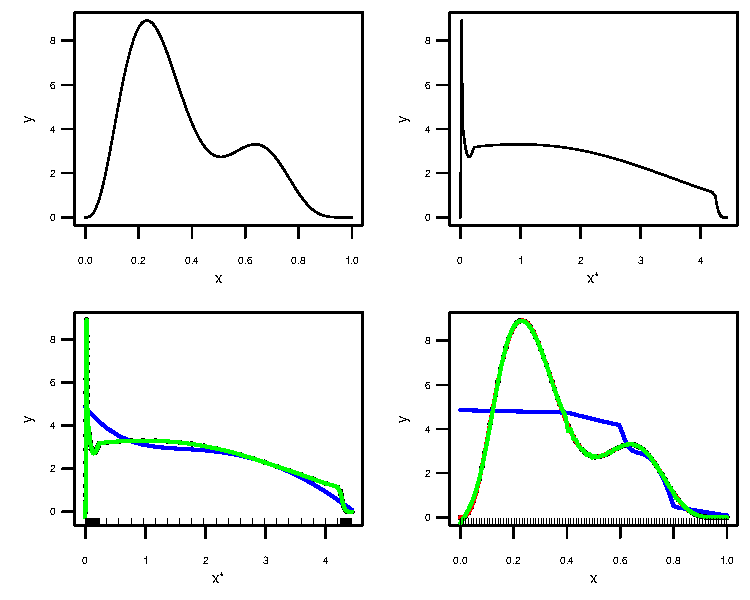
\includegraphics[width=6in]{mds/figs/1dadjust.pdf} \\
\caption{Using penalty adjustments to fit a regression spline to \eqn{hardfcn} after it has been squashed. The function in the top left is squashed to the form in the top right. The bottom left plot shows the fit from a \tprs\ (blue) and a \tprs\ with adjusted penalty (green) in the transformed space. The bottom right shows the same fit in the untransformed space. Clearly, the penalty adjustment improves the fit.}
\label{1dadjust}
% generated by thesis/mds/figs/tpintexp.R
\end{figure}

\subsubsection{Penalty adjustment calculation}

For the moment let us take $\hat{f}$ to be a one dimensional smooth function. It may be decomposed into its basis functions and coefficients in the usual way:
\be
\hat{f}(x)=\sum_{j=1}^J \hat{\beta}_j b_j(x) = \tr{\hat{\bm\beta}}\bm{b}(x).
\ee
The $ij^\text{th}$ element of the penalty matrix (see \secref{GAMpenalties}) is given as:
\be
S_{ij}= \int_a^b \mathcal{L}^*(x) \frac{\partial^2 b_i(x)}{\partial x^2}\frac{\partial^2 b_j(x)}{\partial x^2} \text{d}x = \int_a^b \mathcal{L}^*(x) b^{\prime\prime}_i(x) b^{\prime\prime}_j(x) \text{d}x,
\ee
in one dimension (letting a prime indicate differentiation with respect to $x$). The integral can then be approximated by the midpoint rule as:
\be
S_{ij}= \frac{b-a}{K}\sum_{k=1}^K \mathcal{L}^*(x_k) b^{\prime\prime}_i(x_k) b^{\prime\prime}_j(x_k) \quad \text{for} \quad x_k=a+\frac{(k-0.5)(b-a)}{K},
\label{midpointS}
\ee
for $k=1,\dots, K$. Second derivatives are evaluated by finite differences in the usual manner:
\be
\label{bfinitediff}
b^{\prime\prime}_i(x) = \frac{ b_i(x+2\epsilon) - 2b_i(x+\epsilon) + b_i(x)}{\epsilon^2}.
\ee
For the sake of efficiency, we in fact calculate a $K\cross J$ matrix $D$ with $kj^\text{th}$ element:
\be
D_{kj}=\sqrt{\mathcal{L}^*(x_k)} b^{\prime\prime}_j(x_k),
\label{oneDD}
\ee
for $x_k$ as above. Then $S$ may be calculated as:
\be
S=\frac{b-a}{K}\tr{D}D.
\ee

In this example $\mathcal{L}^*(x)$ was simply calculated using the inverse of the cube of the factor by which the relevant part of the domain (given above) was squashed. 

\subsubsection{Checking that the adjustment works}

\Fig{1dadjust} shows that the adjustment faithfully repdroduces $g(x)$ for the zero error case, fitting a much more sensible model than the standard \tprs. To check that this is true more generally, $\lambda$ was specified (rather than being automatically selected) so that the models with modified and unmodified penalties would have the same EDF. \Fig{1dedfdia} shows such an experiment. Using \eqn{hardfcn} with Normal(0, 0.4) noise added the smoothing parameter was set so that the EDF would be 71, 19 and 42 (working down the diagram). The plots show that the adjustment deviates from truth at most as badly as the vanilla \tprs\ but overall corrects some of the departures from the truth, even in presence of error with a restricted basis.

% 1d adjustment EDF comparison diagram
\begin{figure}
\centering
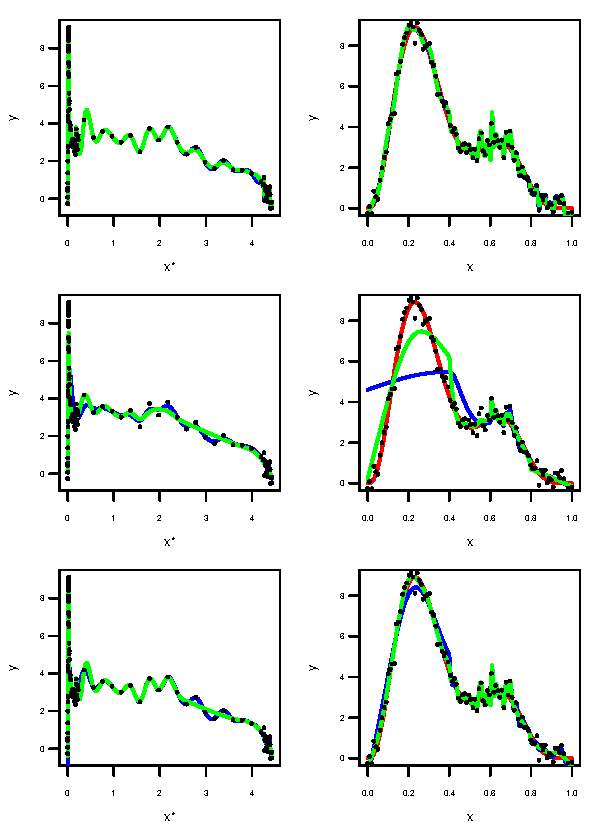
\includegraphics[width=5.5in]{mds/figs/1dedfdia.pdf} \\
\caption{Predictions in transformed and untransformed (left and right columns respectively) for \tprs\ (blue line) and penalty adjusted \tprs\ (green line) fits to the function in \eqn{hardfcn} when the smoothing parameter was pre set to give EDF of 71, 19, and 42 (top to bottom).}
\label{1dedfdia}
% generated by thesis/mds/figs/tpintexp.R
\end{figure}


\subsection{Penalty adjustments in two dimensions}

Using a similar procedures as for one dimension, the two dimensional case can be addressed. Again looking at the $ij^\text{th}$ element of $S$, for the two dimensional case we have:
\begin{equation}
S_{ij}=\int\int_\Omega \mathcal{L}^*(x,y) \Big( \frac{\partial^2 b_i(x,y)}{\partial x^2}\frac{\partial^2 b_j(x,y)}{\partial x^2}+2\frac{\partial^2 b_i(x,y)}{\partial x \partial y}\frac{\partial^2 b_j(x,y)}{\partial x \partial y}+\frac{\partial^2 b_i(x,y)}{\partial y^2}\frac{\partial^2 b_j(x,y)}{\partial y^2} \Big) \text{d}x\text{d}y.
\end{equation}
Matrices analogous to \eqn{oneDD} can be constructed using the finite differences from \eqn{bfinitediff} for differentials $x$ and $y$ individually and
\be
\frac{\partial^2 b_i(x,y)}{\partial x \partial y} = \frac{ b_i(x+\epsilon,y+\epsilon) - b_i(x+\epsilon,y) - b_i(x,y+\epsilon) + b_i(x,y)}{\epsilon^2},
\ee
for the cross term. The matrices then take the form:
\be
[D_x]_{kj}=\sqrt{\mathsf{K}(x_k,y_k)} \frac{\partial^2 b_j(x_k,y_k)}{\partial x^2},
\ee
\be
[D_y]_{kj}=\sqrt{\mathsf{K}(x_k,y_k)} \frac{\partial^2 b_j(x_k,y_k)}{\partial y^2},
\ee
\be
[D_{xy}]_{kj}=\sqrt{\mathsf{K}(x_k,y_k)} \frac{\partial^2 b_j(x_k,y_k)}{\partial x \partial y}.
\ee
So we may then express $S$ as:
\be
S=\tr{D_x}D_x + \tr{D_{xy}}D_{xy} + \tr{D_y}D_y.
\ee
Where the partial derivative evaluation points ($x_k$ and $y_k$) now form a grid for the integration to be calculated. First defining $x^\dagger_k$ and $y^\dagger_k$ analogously to \ref{midpointS}, we have:
\be
x^\dagger_k=a_x+\frac{(k-0.5)(b_x-a_x)}{K},\\
y^\dagger_k=a_y+\frac{(k-0.5)(b_y-a_y)}{K},
\ee
for $k=1,\dots,K$. The integration grid may then be constructed as:
\be
\{x_k : k=1,\dots,K\} = \{x^\dagger_1,x^\dagger_1,x^\dagger_1,\dots, x^\dagger_2, x^\dagger_2, x^\dagger_2,\dots, x^\dagger_K, x^\dagger_K, x^\dagger_K\},
\ee
\be
\{y_k : k=1,\dots,K\} = \{y^\dagger_1,y^\dagger_2, y^\dagger_3,\dots, y^\dagger_K,y^\dagger_1,y^\dagger_2, y^\dagger_3,\dots, y^\dagger_K,\dots\}.
\ee
Finally, those $(x_k,y_k)$ that do not lie inside the boundary in MDS space are removed leaving only those points that lie inside.

\subsubsection{Finding $\mathcal{L}^*$}

Calculating $\mathcal{L}^*(x,y)$ in two dimensions is more tricky than in the one dimensional case. Since the two-dimensional case is to be used in practise, the method for finding $\mathcal{L}^*(x,y)$ must depend on the MDS configuration, as the stretch factors will not be known \emph{a priori} (as was the case in the previous example).

The general idea is to make $\mathcal{L}^*(x,y)$ a function of the change in density of points caused by projecting the original space into MDS space. However, if we assume that the density in the untransformed space is $1$ everywhere, we merely need to calculate the density in MDS space. Having calculated the point density in MDS space, $\mathcal{L}^*(x,y)$ is just some function of this density.

In order to find calculate the point density in MDS space, the following steps are performed:

\begin{enumerate}
\item A grid in the original space is mapped into the MDS space. Ideally, this grid would be dense enough for it to be possible to just count the number transformed points in each square of a regular mesh. However, it would be computationally demanding to project a dense grid into MDS space, so instead a sparse grid is used and then interpolated. This consisted of taking 10 equally spaced points on each side of the square and drawing lines between points on opposing sides. Where the lines crossed were the extra points (along with those points lying on the boundary of the square itself).
\item The interpolated points are then used to estimate the overall point density in MDS space by simply counting the number of points there were in each of a set of squares made from the integration grid, call is $\mathcal{L}(x,y)$. This is shown in \fig{densgrid} for the double peninsulae domain. 
\item Then define $\mathcal{L}^*(x,y)$ as the function
\be
\mathcal{L}^*(x,y)=\frac{1}{(1+\mathcal{L}(x,y))^{3/2}}.
\ee
The $+1$ in the denominator ensures that we do not divide by zero when evaluating $\mathcal{L}^*(x,y)$. The fact that $\mathcal{L}^*(x,y)$ is then a piecewise function should not be too worrying since the aim here is to address the broader problems with the change in spatial density, not the fine-gained details.
\end{enumerate}

Note that the power is now $\frac{3}{2}$. This is since we do not know the contraction/expansion in each direction individually, but rather the overall change in area. As such we use $\frac{3}{2}$ rather than the cubic on $x$ and $y$ and unitary on the cross term.

\begin{figure}
\centering
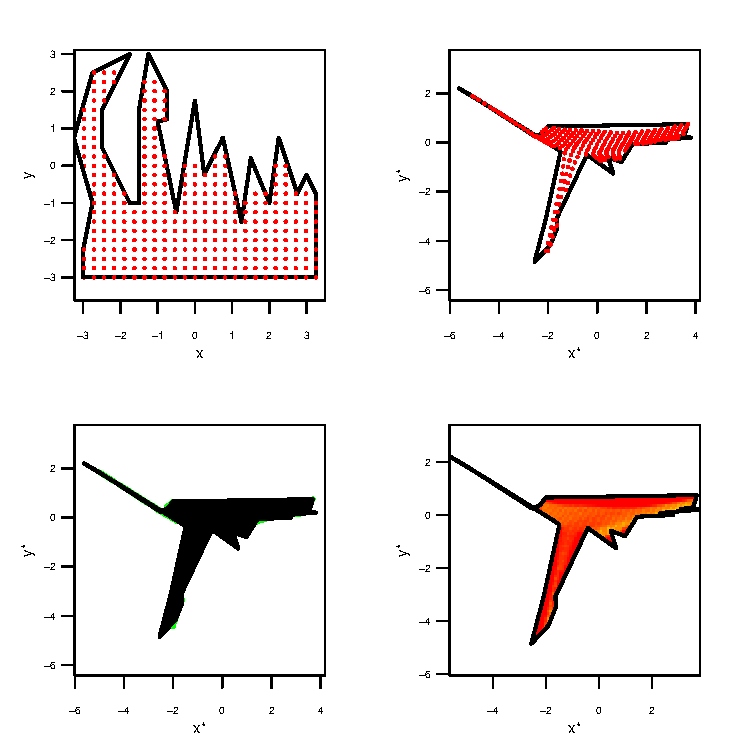
\includegraphics{mds/figs/densgrid.pdf} \\
\caption{The grids used to calculate $\mathcal{L}^*(x,y)$ for the double peninsulae domain. The red grid in the top left figure is mapped to the red grid in the top right panel. The red points in the top right are then used as the basis for the interpolation in the bottom left. The number of green points in each of the squares made from the black points in the bottom left plot are used to calculate the spatial density in that square. The heat map in the bottom right shows the values of $\mathcal{L}(x,y)$ (ie. the density of the green points), here red is low density, yellow is high. Note that some of the points lie outside of the boundary in the MDS projections. This is due to the boundary in MDS space being the straight line interpolant of the vertices of the boundary in the original space.}
\label{densgrid}
% generated by phd-smoothing/mds/wt2-intexp.R and intexp/smooth2.c.R with comments removed
\end{figure}

\subsubsection{Checking that the adjustment works}

In order to make sure that the adjustment works in both the known and unknown contraction/expansion case, a small simulation was run. In this case a surface consisting of two bivariate Normal distributions (mean vectors $(0,-0.5)$ and $(0,0.5)$, covariance matrix diagonal entries $(0.2,0.1)$) were sampled from (sample size 300) and then noise added from a $\text{Normal}(0,0.05)$ distribution. The surface was then divided into its four constituent quadrants about the origin and squashed according to the following factors (in $(x,y)$ pairs, in order top left, top right, bottom left, bottom right): ((0.3,5),(1,5),(0.3,1),(1,1)).

The samples were then used to fit a standard \tprs\ model, \tprs\ with adjusted penalty with known stretch factors and a \tprs\ with $\mathcal{L}^*(x,y)$ estimated from the data. The mean squared error between the truth and prediction over a dense (50 by 50) grid was then calculated.

The simulation results show that there is a decrease in MSE when the expansion/contraction of the space is taken into account (MSEs were: $2.355, 2.300 \text{and} 2.305$ for \tprs, known stretch and estimated stretch, respectively). Unfortunately this didn't offer the same visual improvement as the 1-dimensional case, so heat maps are not shown here.

The next section puts the adjusted penalty approach to the test on a number of domains and compares it to other possible models.

\subsection{Wider simulations and real data}

\subsubsection{Peninsulae domain}
\label{wt2bigsim}

Using the same setup as in \secref{mds-wt2-sim}, for each error level ($\sigma=0.35, 0.9, \text{ and } 1.55$), 200 realisations were generated. From these 250 samples were drawn to fit the model, predictions were made over a grid of 1253 points with MSE and EDF recorded per model for each simulation. 

The models that were fitted were:
\begin{enumerate}
\item \emph{TPRS}: \tprs\ with basis size 140.
\item \emph{MDS+TP}: \mdsap\ using a \tprs\ with basis size 140.
\item \emph{MDS+CR}: \mdsap\ using a tensor product (see \secref{GAMtensor}) of two cubic regression splines, each dimension of which had a basis size of 12.
\item \emph{MDS+3D}: \mdsap\ using a 3-dimensional \tprs\ with basis size 140. Here MDS was used to project the data into three dimensions rather than two.
\item \emph{MDS+ADJ}: \mdsap\ using a \tprs\ with basis size 140, with penalty adjustments.
\item \emph{Soap film smoother}: using 109 internal knots evenly spaced on a grid over the domain, with boundary basis size 60.
\end{enumerate}

As can be seen in \tabref{bigwt2resultstable}, the results from MDS+ADJ are actually worse than those from just MDS+TP in all but the lowest noise case. \Fig{big-wt2-mses} shows box plots of these results.

However, all is not lost, MDS+3D and MDS+CR are competitive across the board, beating the soap film smoother in some cases. For the cubic regression spline, this is probably due to the tensor setup of the spline. Having a different smoothing parameter for each direction will allow the model to take care of the anisotropic space into which the data has been projected. In the high noise case the MDS+TP has a lower and less variable MSE than MDS+CR, this may well be due to the \tprs\ enforcing the isotopy in a high-noise case and this constraint has lead to a less wiggly model being fitted, which happens to be closer to the truth in this case. As for the 3-D projection, the plots in \fig{wt2-3d-proj} show that the additional dimension allows for further separation of both a large and small peninsulae, which should help with the anisotropy as well as leakage.

A Wilcoxon signed rank test, matching pairs between realisations showed that there was a significant difference between the MSE of each model and the soap film smoother. As can be seen from \fig{big-wt2-mses}, soap outperforms all of the other methods on this domain, with MDS+3D coming in second. 

Finally, note that there were three realisations omitted (for all models) in \tabref{bigwt2resultstable} and \fig{big-wt2-mses}. In these realisations the soap film smoother failed to fit the model due to knot placement. These can be safely removed as, in practise, the computer would inform the user that the knot placement was not appropriate and the knot layout could be altered.

\begin{sidewaystable}[p]
\centering
\begin{tabular}{c c c c c c c}
 & &  & MSE  & & &\\ 
$\sigma$  & tprs & mds+tp & mds+cr & mds+tp 3D & mds+tp+adj & soap\\ 
\hline
0.35  & 0.0832 (1e-04) & 0.0713 (5e-05) & 0.0633 (8e-05) & 0.0579 (5e-05) & 0.0697 (5e-05) & 0.0598 (0.00032) \\ 
0.9  & 0.1957 (0.00017) & 0.1788 (0.00013) & 0.1651 (0.00025) & 0.1478 (0.00014) & 0.1875 (0.00017) & 0.1616 (0.00201) \\ 
1.55  & 0.3576 (0.00035) & 0.285 (0.00027) & 0.3196 (0.00063) & 0.2765 (0.00032) & 0.3509 (4e-04) & 0.245 (0.00034) \\
\end{tabular}
\begin{tabular}{c c c c c c c}
 & &  & EDF  & & &\\ 
$\sigma$  & tprs & mds+tp & mds+cr & mds+tp 3D & mds+tp+adj & soap\\ 
\hline
0.35  & 77.8675 (0.03803) & 80.5454 (0.04111) & 53.9125 (0.03577) & 61.3458 (0.05324) & 73.3275 (0.03707) & 55.2464 (0.04684)\\ 
0.9  & 47.0214 (0.0378) & 34.357 (0.05645) & 31.9157 (0.03525) & 30.5807 (0.04027) & 40.409 (0.03805) & 29.6874 (0.04514) \\
1.55  & 31.8803 (0.03843) & 18.3575 (0.03865) & 20.4563 (0.04242) & 19.7871 (0.03128) & 26.6778 (0.03572) & 20.3529 (0.03171)\\ 
\end{tabular}
\caption{Mean MSE and EDF for the six models fitted to the peninsula domain with standard errors (in brackets) over 197 realisations.}
\label{bigwt2resultstable}
\end{sidewaystable}

% big wt2 sim MSEs
\begin{sidewaysfigure}
\centering
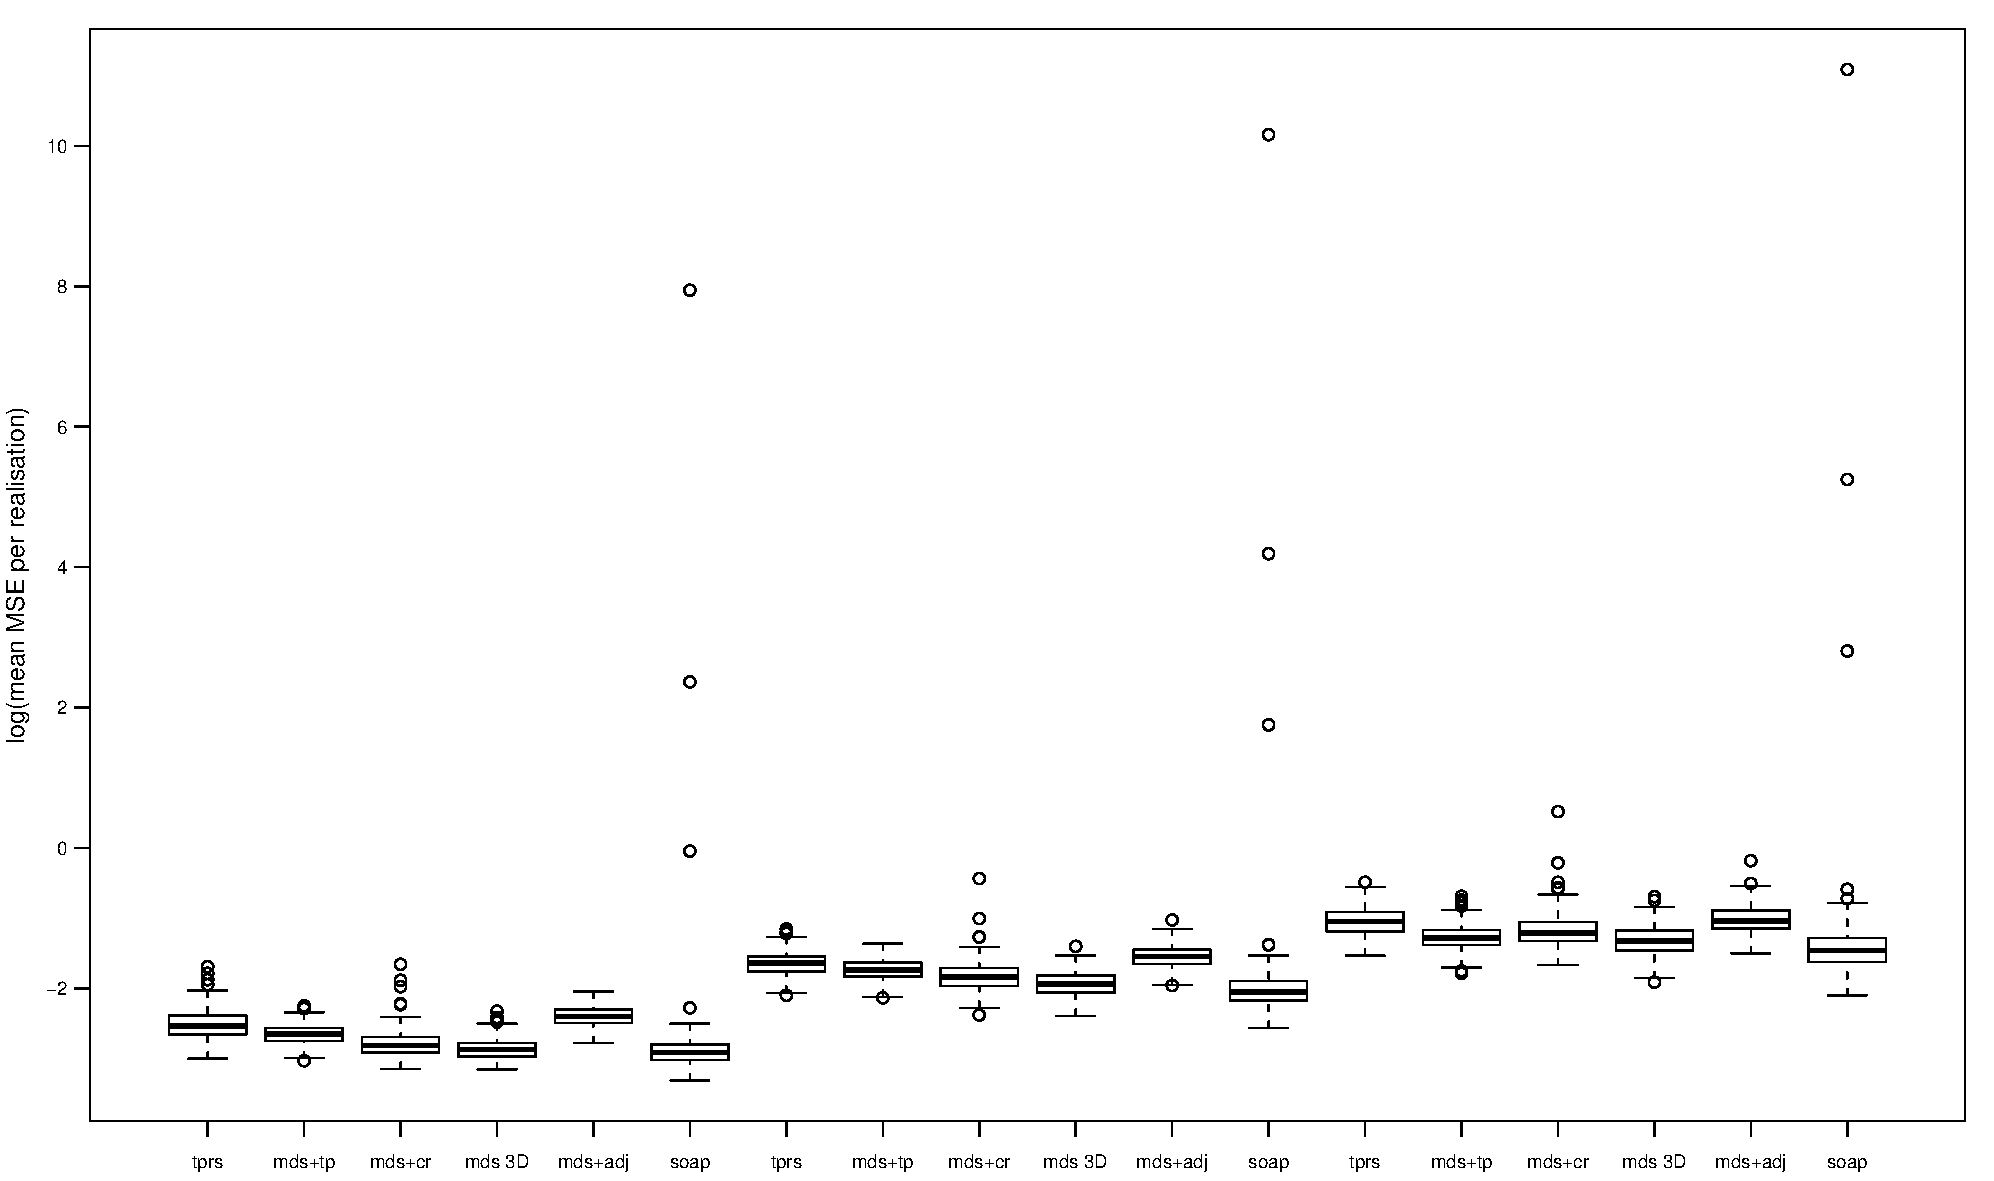
\includegraphics[width=9.5in]{mds/figs/big-mds-wt2-boxplot.pdf} \\
\caption{Logarithm of per realisation average mean squared error for the double peninsulae domain. Models are in groups of six for each error level ($\sigma=0.35,0.9,1.55$). In all cases, a Wilcoxon signed rank test showed that MSEs for all models were significantly different from the soap film smoother ($\text{p-value} < 10^{-6}$).}
\label{big-wt2-mses}
% generate /phd-smoothing/mds/sim/boxplot-wt2.R
\end{sidewaysfigure}


\subsubsection{Aral sea}

The Aral sea is located between Kazakhstan and Uzbekistan. It has been steadily shrinking since the Soviet government diverted the sea's two tributaries in order to irrigate the surrounding desert during the 1960s. The NASA SeaWifs satellite collected data on chlorophyll levels in the Aral sea (\cite{soap}). The 496 data are averages of the $38^\text{th}$ 8 day observation period over the years 1998 to 2002. Smooths were fitted to the spatial coordinates (Northings and Easting projected from latitude and longitude) with the logarithm of chlorophyll concentration (with Gamma errors) as the response.

A \tprs, \mdsap\ and soap film were all fitted to the data. In summary the setup for each model was:

\begin{enumerate}
\item \emph{Thin plate spline}:  with basis size 70.
\item \emph{Soap film smoother}: using a 12 by 12 grid of knots (74 were inside) and a boundary smooth with basis size 49.
\item \emph{\mdsap}: \tprs\ with basis size 70.
\end{enumerate}

\begin{figure}
\centering
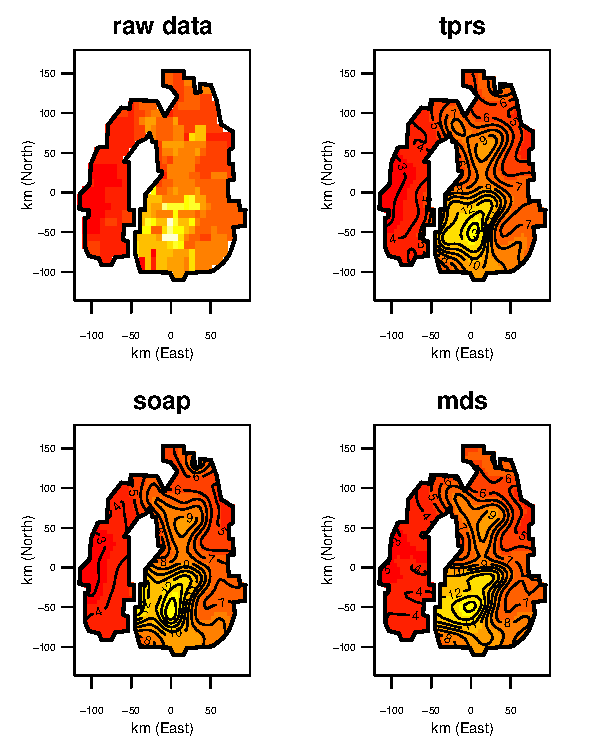
\includegraphics{mds/figs/aral-fit.pdf} \\
\caption{Raw data and predictions from the models fitted to the Aral sea chlorophyll data. Clockwise from top left: raw data, \tprs, soap film smoother, and \mdsap.}
\label{aral-fit}
% generated by phd-smoothing/mds/wt2-intexp.R and intexp/smooth2.c.R with comments removed
\end{figure}

The models were then used to predict over a grid of 496 points to create the heat maps shown in \fig{aral-fit}. The fits are broadly similar, with the \tprs\ showing some signs of leakage around (-50,-50). Both \mdsap\ and the soap film smoother combat this problem. The contour lines for all of the models look roughly the same in the main part of the sea, but in the smaller lobe, \mdsap\ is rather different from both the soap film and \tprs. 

Although the leakage is avoided, there appear to be some strange artefacts in the smooth. Ovals of higher chlorophyll appear in the smaller lobe when the \mdsap\ is fit to the data, along with contours close to the far left of the smaller lobe. Looking at a point plot in MDS space (\fig{aral-pp}) reveals why this might be happening. As can be seen from the figure, the smaller lobe has been severely squashed which will clearly have an adverse effect on the smoother.

\begin{figure}
\centering
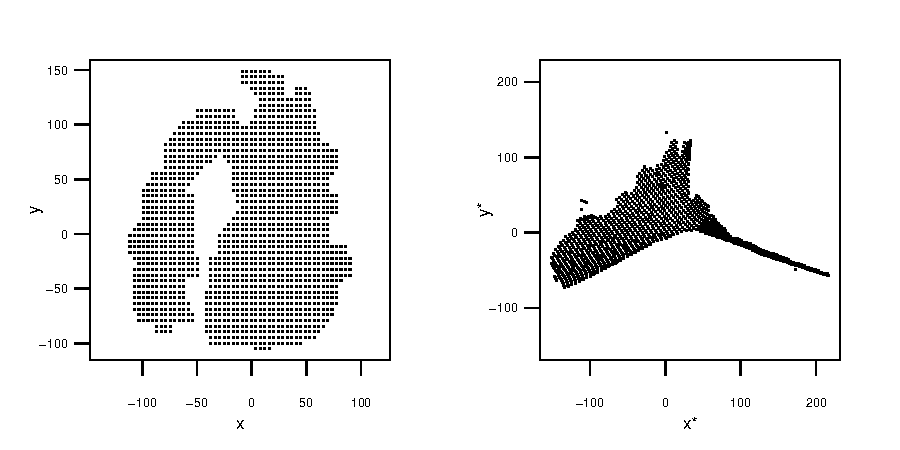
\includegraphics[width=6.25in]{mds/figs/aral-pp.pdf} \\
\caption{The prediction points for the Aral sea data set (left), with their projection into MDS space (right).}
\label{aral-pp}
% generated by phd-smoothing/mds/aral/pointplot.R
\end{figure}

The \mdsap\ with adjusted penalty was also used to fit the model, using the same basis as above. The predicted surface given by the model is shown in \fig{aral-adj-fit}. Again, the same artefacts are clearly visible in the smaller lobe of the region.

\begin{figure}[t]
\centering
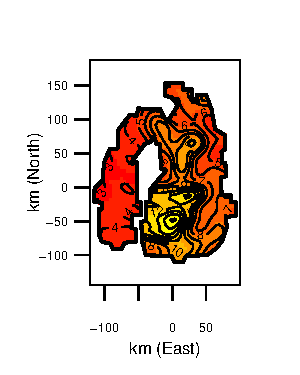
\includegraphics[width=3in]{mds/figs/aral-adjfit.pdf} \\
\caption{Predictions for the Aral sea using \mdsap\ with adjusted penalty.}
\label{aral-adj-fit}
% generated by phd-smoothing/mds/wt2-intexp.R and intexp/smooth2.c.R with comments removed
\end{figure}

Using a 3-D \tprs\ the artefacts are less prominent and the surface looks much more like the one given by the soap film smoother. Again, the three-dimensional projection shows much promise especially given the minimal extra cost to running the additional model (if the within-area distances are already calculated, only the MDS projection needs to be calculated, and the \tprs\ fitted).

\begin{figure}
\centering
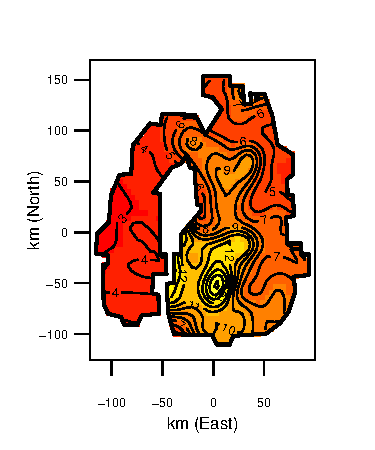
\includegraphics[width=3in]{mds/figs/aral-3d.pdf} \\
\caption{Predictions for the Aral sea using a 3 dimensional projection into MDS space for \mdsap.}
\label{aral-fit-3d}
% generated by phd-smoothing/mds/wt2-intexp.R and intexp/smooth2.c.R with comments removed
\end{figure}

\subsubsection{Aral sea simulation}
\label{mds-aral-sea-sim}

The results above show that \mdsap\ does not fit an unreasonable model, but that some artefacts do occur in the predictions. In order to further test \mdsap, a simulation was setup. Truth was set as the predictions given by fitting a kernel regression (using the \textsf{R} package \texttt{np}) to the raw data in \fig{aral-fit}. Bandwidth was selected by expected Kullback-Leibler cross-validation (\cite{hurvich}) using adaptive nearest-neighbours. A local-linear kernel regression estimator was used. 

Taking this kernel estimate as truth (see \fig{aral-np}), samples of size 100, 250 and 500 were taken and noise added from the Gamma distribution with signal-to-noise ratios 0.95, 0.75 and 0.5 (dispersion equal to 6.666,1.265 and 0.9523, and scale equal to  0.4077, 2.495 and 5.748, respectively). Predictions were then made on a grid 1498 points, from this MSEs were calculated and EDFs recorded for each model over 100 realisations.

\begin{figure}
\centering
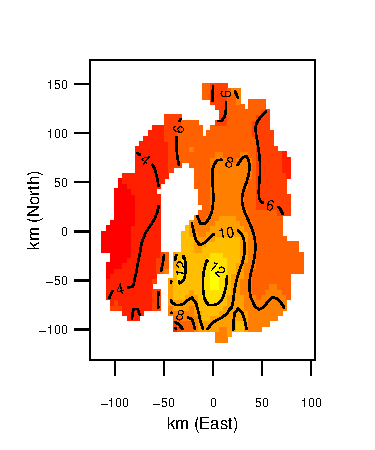
\includegraphics[width=3in]{mds/figs/aral-np.pdf} \\
\caption{The fit given by the kernel regression for the Aral sea, used as truth for simulations in \secref{mds-aral-sea-sim}.}
\label{aral-np}
% generated by thesis/mds/figs/aral-np.R
\end{figure}

The models fitted were as in \secref{wt2bigsim} (but with different basis sizes):

\begin{enumerate}
\item \emph{TPRS}: \tprs\ with basis size 70.
\item \emph{MDS+TP}: \mdsap\ using a \tprs\ with basis size 70.
\item \emph{MDS+CR}: \mdsap\ using a tensor product (see \secref{GAMtensor}) of cubic splines, each dimension of which had a basis size of 9.
\item \emph{MDS+3D}: \mdsap\  using a 3-dimensional \tprs\ with basis size 70. Here MDS was used to project the data into three dimensions rather than two.
\item \emph{MDS+ADJ}:  \mdsap\ using a \tprs\ with basis size 70, with penalty adjustments.
\item \emph{Soap film smoother}: using 74 internal knots evenly spaced on a grid over the domain, and a cyclic spline on the boundary of basis size 25.
\end{enumerate}

% big aral sim MSEs
\begin{figure}
\centering
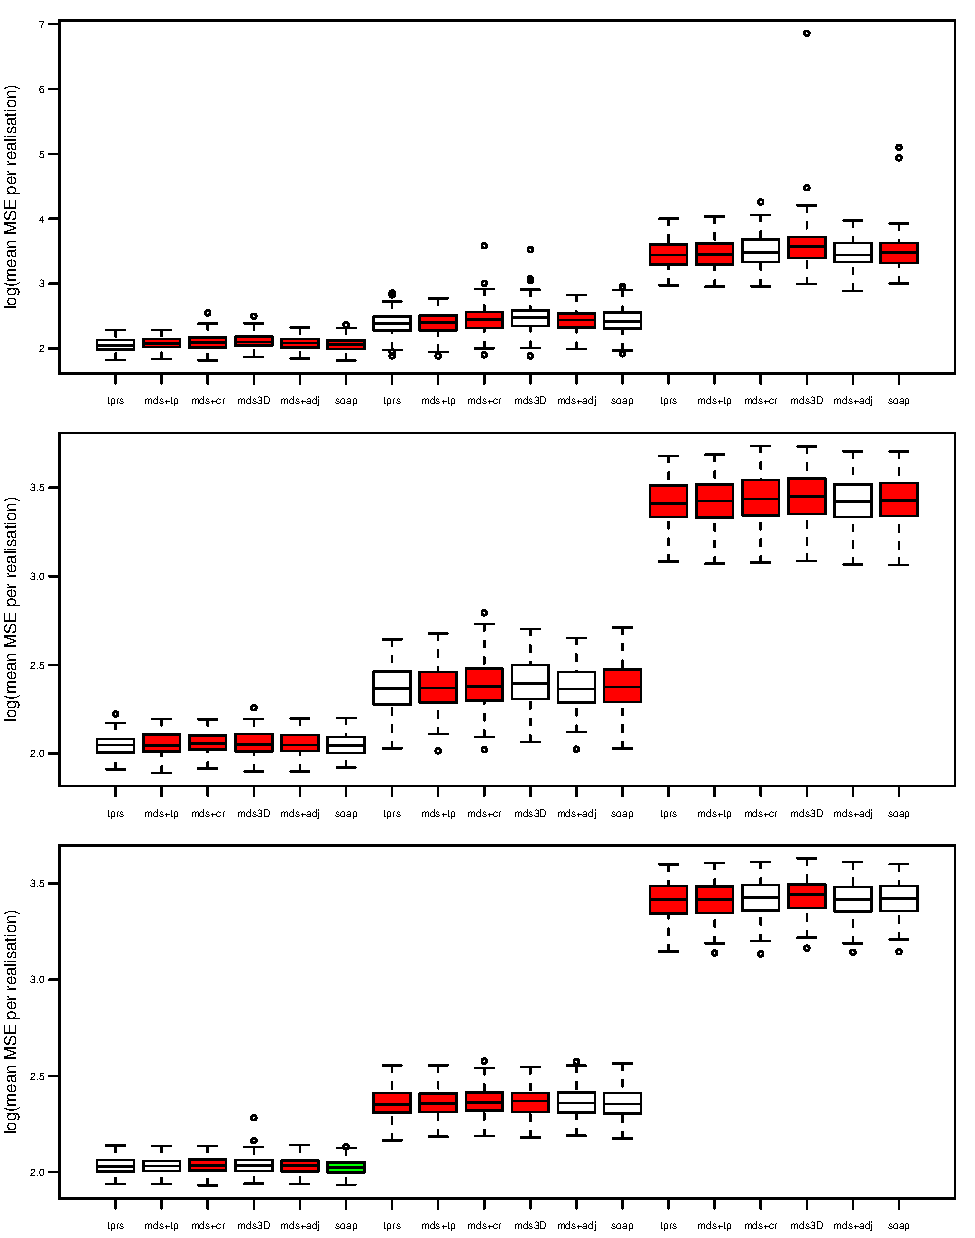
\includegraphics[width=6in]{mds/figs/big-aral-boxplot.pdf} \\
\caption{Box plots of the logarithm of per realisation average mean squared error for the Aral sea simulation. Top to bottom sample sizes: 100, 250, 500. Models are in groups of six for each signal-to-noise ratio (0.95,0.0.75,0.5). The shaded boxes indicate that a Wilcoxon signed rank test showed that there was a significant difference between the model and the \tprs\ MSEs ($\text{p-value} < 10^{-2}$). Red indicates that the model was significantly different and worse (ie. significantly higher MSE than the \tprs), green that it was significantly different and better (ie. significantly lower MSE than the \tprs).}
\label{big-aral-mses}
% generate /phd-smoothing/mds/aral/boxplots.R
\end{figure}

\Fig{big-aral-mses} and \tabref{bigaralresultstable} show the results of the simulations. Looking at these, there does not appear to be a clear reason to choose one of the \mdsap\ methods over the others on MSE grounds alone. Perhaps surprisingly, the \tprs\ does rather well in MSE terms, having slightly lower MSE than other models in almost all situations. This is perhaps to be expected given the leakage was rather slight and localised, this combined with the \tprs\ also fitting a consistently more complex model (see EDFs, \tabref{bigaralresultstable}) may account for the superior MSE. However, we still must prefer the soap film smoother, since it does not allow any leakage. Given the evidence, above, of possible artefacts in \mdsap\ models, the soap film appears to be the best option for smoothing over regions with complex boundaries.

\begin{sidewaystable}[p]
\centering
\begin{tabular}{c c c c c c c c}
 & & &  & MSE  & & &\\ 
 $n$ & SNR & tprs & mds+tp & mds+cr & mds+tp 3D & mds+tp+adj & soap\\ 
\hline
100  &  0.95  & 7.9015 (0.08013) & 7.959 (0.07539) & 8.142 (0.09235) & 8.3365 (0.09319) & 7.9099 (0.07207) & 7.9862 (0.08923) \\ 
100  &  0.75  & 11.1357 (0.20472) & 11.2689 (0.20631) & 11.9138 (0.25673) & 12.2517 (0.24506) & 11.1778 (0.20201) & 11.5665 (0.21725) \\ 
100  &  0.5  & 32.3312 (0.71517) & 32.8335 (0.74064) & 36.3542 (1.82936) & 44.9118 (3.94612) & 32.5586 (0.67499) & 34.7731 (1.59728) \\ 
250  &  0.95  & 7.5986 (0.04417) & 7.698 (0.04591) & 7.7376 (0.04951) & 7.8235 (0.09169) & 7.8895 (0.05065) & 7.6292 (0.04719) \\ 
250  &  0.75  & 10.3526 (0.11208) & 10.5199 (0.11666) & 10.7282 (0.12681) & 10.7975 (0.13027) & 10.9595 (0.12346) & 10.5495 (0.11691) \\ 
250  &  0.5  & 31.1509 (0.4722) & 31.3645 (0.48343) & 32.2298 (0.60102) & 32.6544 (0.54744) & 30.966 (0.40946) & 31.6147 (0.50458) \\ 
500  &  0.95  & 7.6029 (0.03234) & 7.6871 (0.03205) & 7.7303 (0.03395) & 7.6631 (0.03548) & 7.6909 (0.03071) & 7.6072 (0.03209) \\ 
500  &  0.75  & 10.2918 (0.08406) & 10.4119 (0.08297) & 10.5134 (0.08788) & 10.6015 (0.11156) & 10.6991 (0.08454) & 10.373 (0.08497) \\ 
500  &  0.5  & 30.4475 (0.26024) & 30.6894 (0.26375) & 31.0089 (0.26704) & 31.3011 (0.2788) & 30.6516 (0.27123) & 30.8032 (0.26491) \\ 
\end{tabular}
\begin{tabular}{c c c c c c c c}
 & &  & EDF  & & &\\ 
$n$ & SNR & tprs & mds+tp & mds+cr & mds+tp 3D & mds+tp+adj & soap\\ 
\hline
100  &  0.95  & 29.552 (0.87023) & 21.9038 (0.67106) & 18.7032 (0.53711) & 23.254 (0.72225) & 17.3514 (0.45505) & 24.6145 (0.7117) \\ 
100  &  0.75  & 19.491 (0.98279) & 12.8962 (0.56278) & 12.0983 (0.52548) & 13.7002 (0.43143) & 10.6921 (0.34023) & 14.9221 (0.68537) \\ 
100  &  0.5  & 16.5053 (0.91097) & 11.9996 (0.94359) & 11.4546 (0.70547) & 13.7607 (0.51774) & 8.4233 (0.57631) & 12.9575 (0.69218) \\ 
250  &  0.95  & 40.9612 (0.51131) & 33.658 (0.51015) & 28.0043 (0.5445) & 37.5377 (0.63347) & 31.8296 (0.62748) & 38.2715 (0.67473) \\ 
250  &  0.75  & 24.6507 (0.68571) & 19.0361 (0.58564) & 17.6928 (0.64489) & 20.3174 (0.72174) & 17.2911 (0.74521) & 23.2137 (0.76245) \\ 
250  &  0.5  & 19.296 (0.89548) & 14.987 (0.67186) & 12.9415 (0.46289) & 15.3412 (0.6208) & 11.6872 (0.61843) & 18.3504 (1.03563) \\ 
500  &  0.95  & 50.1375 (0.39114) & 43.9809 (0.40286) & 36.0768 (0.57957) & 49.2601 (0.48478) & 42.8032 (0.44318) & 49.6045 (0.76866) \\ 
500  &  0.75  & 31.6271 (0.6354) & 26.8581 (0.72752) & 23.1292 (0.76395) & 29.2308 (0.69282) & 24.762 (0.92098) & 30.0555 (0.7023) \\ 
500  &  0.5  & 25.1535 (0.81385) & 20.7569 (0.89395) & 16.7635 (0.71303) & 20.9786 (0.91157) & 15.8003 (0.79458) & 23.2793 (1.01832) \\ 
\end{tabular}
\caption{Mean MSE and EDF for the six models fitted for the Aral sea simulation with standard errors (in brackets) over 100 realisations.}
\label{bigaralresultstable}
\end{sidewaystable}





\rule{6in}{1pt}
\begin{center}
\textbf{CUT HERE AND EDIT TO INCLUDE DUCHON SPLINES}
\textbf{be careful with labels!}
\end{center}

\section{Problems with the methodology so far}
\label{mds-problems}

\textbf{Some intro blurb goes here}

Left with several problems here, they are

penalty adjustment problems
	ordering
	guarantee of separation

nullspace size



\subsection{Why adjusting the penalty is not the solution}
\label{pensuck}

The simulations show that there is no big advantage of using the adjusted penalty scheme for \mdsap\ over the non-adjusted penalty. Before running the simulations, several different functions of the MDS point density were compared. All were worse than the function that was finally settled on.

An explanation for why the penalty adjustment doesn't offer much improvement can be found by investigating the good performance of the 3-D projection model. 

Looking at the plots of the prediction points in MDS space for the peninsulae domain (\fig{wt2-2d-proj} and \fig{wt2-3d-proj}) it is easy to see that in two dimensions, the first peninsula has been squashed to a line. This is a result of the truncation performed to $\tilde{X}^*$ in the MDS procedure (see \secref{MDStechdet}); when we look at the 3-D projection, the peninsula clearly has width, just not in the two dimensional projection. The adjusted penalty attempts to account for this squashing of the points by allowing a more flexible model to be fit in that area. However, what is not taken into account is that some of the points in the peninsula are projected on top of each other or on the wrong side of one another. In other words, the MDS projection makes the points lose their ordering. 

As a simple, unidimensional example, take three points, $a, b, \text{and}\ c$ in the top line of \fig{linedia}. The projection could squash them in the way shown on the second line, in this case the penalty adjustments as described in \cite{wood2000} could be used to correct the model. However, with MDS we can have a situation occurring which is similar to that shown in the bottom line of \fig{linedia}, changing the order of $a, b, \text{and}\ c$. 

In the MDS projection we can see this happening in the peninsula described above. The projection takes a side-on view of the peninsula, making the points lose their ordering. In this case, the penalty adjustment can't save the model. If the ordering of the points is not guaranteed, then the smoother's job is potentially impossible, especially when one thinks of the 2-dimensional extension of \fig{linedia}.

\begin{figure}
\centering
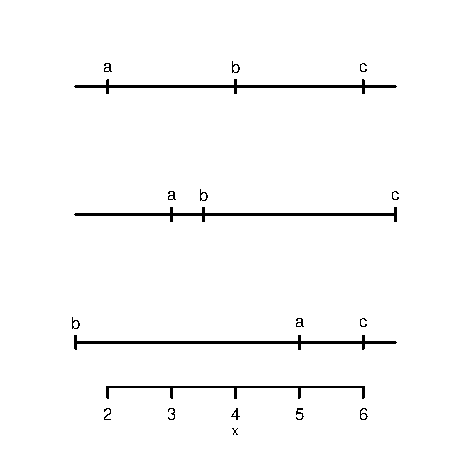
\includegraphics[width=3in]{mds/figs/linedia.pdf} \\
\caption{An illustration of how spatial mappings can squash points (middle line) and reorder them (bottom line) from their original configuration (top line).}
\label{linedia}
% generated by thesis/mds/figs/linedia.R
\end{figure}

In order to test this hypothesis in practise, a simulation was run using the Aral sea (simulation) data set from \secref{mds-aral-sea-sim}. \mdsap\ was fitted to 100 realisations of the domain. However, in order to see if the distortion to the smaller peninsula is problematic, the model was fit in two halves. One half consisted of the smaller peninsula on the left; the other the rest of the domain (splitting on the $-45$ kilometre East line). Models were fitted to each half and predictions made for the halves individually. If there were no problems with the squashing in the left peninsulae then we should find that the MSEs are not significantly different between the two areas (there is no reason that their MSEs should be different, since we add the same amount of error, sample the same number of points and control for leakage by separating the two parts). Using a Wilcoxon signed rank test on paired MSEs, the difference was significant ($\text{p-value} < 10^{-3}$). It therefore seems safe to conclude that this phenomenon causes problems for \mdsap\ when parts of the domain are squashed.

\subsection{Why moving to higher dimensions is not the solution}
\label{nohigherdim}

In the two cases above, moving into three dimensions allowed \mdsap\ to more accurately reproduce the true function. Counteracting the phenomenon above (where the ordering of the points is lost), the extra dimension allows us to see the ``width'' of parts of the domain that we take a side view of in the 2-dimensional projection.

It seems then that there is some milage in taking a 3-dimensional projection to solve this problem without the need for penalty adjustments. However, unfortunately, this is not the case in general. \Fig{mds-comb} shows a long domain with three peninsulae at each end. The MDS projection of the domain in two dimensions gives the points in \fig{mds-comb-2d}. There are only four peninsulae in this figure, not the six which were in the original. Using the colours in \fig{mds-comb} and \fig{mds-comb-2d}, it is clear that the larger peninsulae are separated but not the smaller ones. Assuming that there are some features in the smaller peninsulae and there is reason to believe that leakage would be undesirable, this looks rather bad from a smoothing perspective.

\begin{figure}
\centering
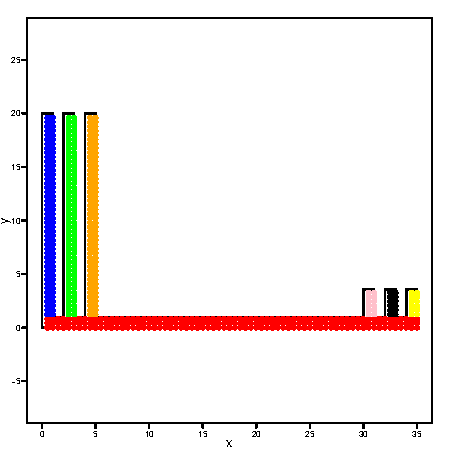
\includegraphics[width=3in]{mds/figs/comb.pdf} \\
\caption{The ``comb'' domain from \secref{nohigherdim}.}
\label{mds-comb}
% generated by thesis/mds/figs/comb.R
\end{figure}

\begin{figure}
\centering
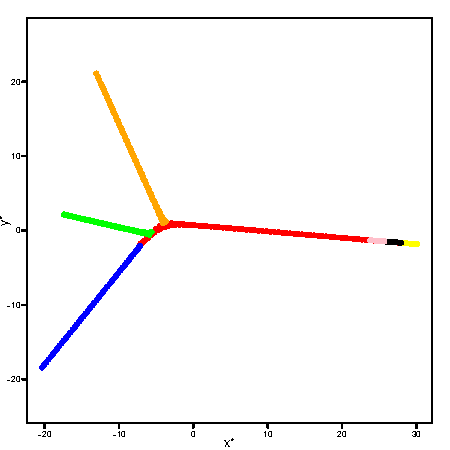
\includegraphics[width=3in]{mds/figs/comb-2d.pdf} \\
\caption{Two-dimensional MDS projection of the domain in \fig{mds-comb}, note that there are only four ``legs'' here not the six that should be there, as in \fig{mds-comb}.}
\label{mds-comb-2d}
% generated by thesis/mds/figs/comb.R
\end{figure}

So, in this case it is not unreasonable to think that an extra dimension could help. Taking a 3-dimensional projection, \fig{mds-comb-3d} is produced; however there is still no separation of the smaller peninsulae. Moving into four dimensions (\fig{mds-comb-4d}) we begin to see separation in the smaller peninsulae. However, even in four dimensions the separation is not particularly large and leakage could still occur.

\begin{figure}
\centering
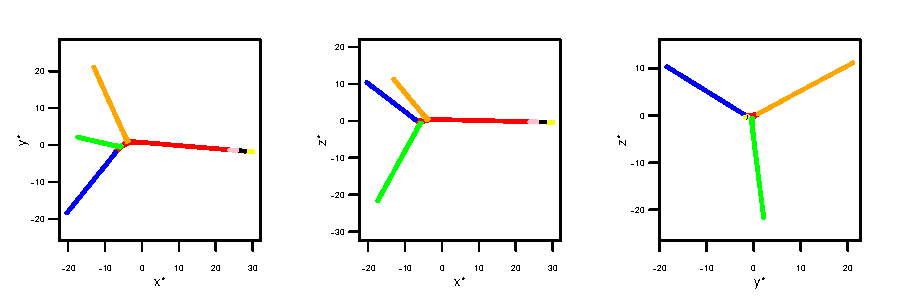
\includegraphics[width=6in]{mds/figs/comb-3d.pdf} \\
\caption{The MDS projection of the domain in \fig{mds-comb} into three dimensions. Note that there is still no separation in for the smaller peninsulae.}
\label{mds-comb-3d}
% generated by thesis/mds/figs/comb.R
\end{figure}

\begin{figure}
\centering
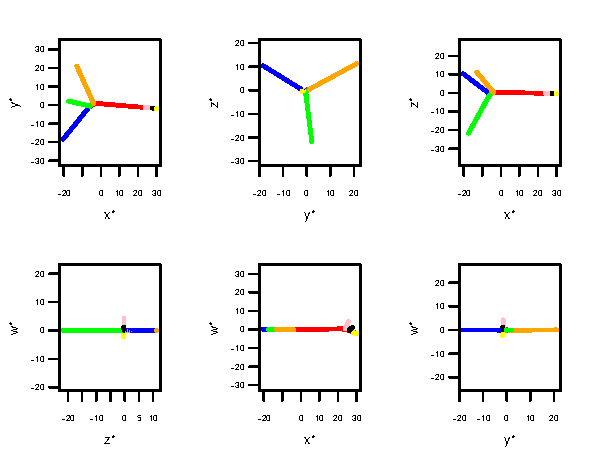
\includegraphics[width=6in]{mds/figs/comb-4d.pdf} \\
\caption{The MDS projection of the domain in \fig{mds-comb} in four dimensions.}
\label{mds-comb-4d}
% generated by thesis/mds/figs/comb.R
\end{figure}


\rule{6in}{1pt}

\rule{6in}{1pt}

\textbf{THINK ABOUT THIS SECTION}
\textbf{Need to keep some of it, but not sure that the quantitative parts are useful.}


Although these plots are illustrative, a quantitative measure of how well the within-area distances are being approximated by the MDS projection is desirable. Given the eigen-decomposition attempts to minimise the spectral norm, this is the logical metric to use. If we label the matrix of within-area distances $D$ (as above) and the matrix of Euclidean distances in MDS space as $D_E$, then we may calculate the spectral norm as the largest eigenvalue of $D-D_E$.

% Results here are in mds/counter/run-DRcomp.R
Looking at this measure for the domain considered in this section (the ``comb''), peninsulae domain (from \secref{mds-wt2-sim}) and the Aral sea as dimension of projection is increased yields some interesting results. These are summarised in \tabref{increasek}. The table indicates that there is some optimum number of dimensions ($k$) to project into, such that adding a further dimension gives only a negligible decrease in the spectral norm. 

However, the optimal $k$ is not common to all of the domains. For the peninsulae domain there is a large decrease (roughly halving each time) up to four dimensions, but the Aral sea appears to settle down after three. However, we can see that this is by no means definitive, given that for the ``comb'' domain, four dimensions appears to be optimal but \fig{mds-comb-3d} shows that this doesn't offer much separation in the peninsulae.

Since there appears to be no particular limit on the number of dimensions to project into in order to get a set of points that avoid both leakage and the ordering problem, it is hard to believe that simply extending to higher dimensions is a sustainable solution.

\begin{table}[htb]
\centering
\begin{tabular}{c c c c c}
$k$ & Comb  & Peninsulae & Aral\\ 
\hline
1  &  3610.210  &  109.1344  &  1519.736 \\ 
2  &  1280.189  &  54.60339  &  347.2212 \\ 
3  &  459.9464  &  22.06782  &  128.2021 \\ 
4  &  457.1626  &  12.16595  &  119.5486 \\ 
5  &  456.0698  &  10.23667  &  117.6430 \\ 
6  &  452.4361  &  9.95791  &  116.6678 \\ 
7  &  450.9335  &  9.873292  &  116.1673 \\ 
8  &  450.5587  &  9.853141  &  115.5955 \\ 
9  &  449.8825  &  9.789696  &  115.3094 \\ 
10  &  449.4629 &  9.746579  &  115.1879 \\ 
\end{tabular}
\caption{Mean squared difference between the matrix of within-area distances and Euclidean distance in a $k$-dimensional MDS projection of the points for each of the domains detailed in \secref{nohigherdim}.}
\label{increasek}
\end{table}

Moving into continually higher dimensions seems appealing, but practically it is rather more taxing. As the dimension of the problem is increased, the order of the penalty in the GAM increases too(see \secref{GAMpenalties}). As this happens, the dimension of the nullspace of the penalty increases, meaning that more functions are unpenalised in the model. This will not lead to a simple model being fitted to the data: the real aim of \mdsap.


\rule{6in}{1pt}

\rule{6in}{1pt}

\section{Reliable high dimensional smoothing using Duchon splines}

The previous section makes clear that there are two conflicting issues impeding the utility of this approach to smoothing over complex regions. The first is that the ordering of the points in space must be maintained, but (second) once a sufficiently high dimensional projection of the data has been obtained, the nullspace of the penalty must be kept as small as possible in order to stop a large space of wiggly function from being fit without being penalised.

Facing the interplay of these two factors, the requirement we seek is clear: we wish to smooth in as many dimensions as possible but while doing this we must also limit the nullspace of the penalty. Fortunately, this is possible using the ideas put forth in \cite{duchon77}. The methods detailed there give a generalisation of the thin plate spline basis that allows for the nullspace to be constrained.

The next subsection goes into the technical detail of how this approach works. Subsequent sections give the practical implications \textbf{add more to this!}

\subsection{blah}
fucking Duchon splines: how do they work?


\begin{equation}
\lVert u \rVert_{m,s} = \Big( \int_{\mathbb{R}^n} \lvert \tau \rvert^{2s} \lvert \mathfrak{F} D^m u(\tau) \rvert^2 \text{d} \tau \Big)^{1/2}
\end{equation}

\subsection{blah}

percent variation


\subsection{blah}

using gcv/ml score to choose k


\subsection{blah}

some simulations


\subsection{blah}

nice smoothed version of aral sea

\subsection{blah}

some stuff about software




\rule{6in}{1pt}

\rule{6in}{1pt}


\section{\mdsap\ in practise}
\label{mds-prac}

\textbf{This can now go at the end, modified for the Duchon splines stuff.}

Although \mdsap\ has problems, there may be some cases in which it is useful. For this reason, some practical tips on using the method are given here.

As has been seen in the previous sections, \mdsap\ does have potential pitfalls for the practitioner. Key to the whole method is that the starting grid, used to project the data into MDS space is dense enough so that the features of the domain which cause leakage are captured. In order to make sure that the initial grid is dense enough, a sparse grid over the boundary could be created and gradually made more dense grids until there are only very small changes in the plot of the grid in MDS space. Automation could be achieved by following a similar process (starting with a sparse grid and increasing the density) and at each stage checking to see if the the eigenvalues of the distance matrix have converged.

Choosing a suitable boundary is also essential to making sure that a model can be fitted in reasonable time. The more complex the boundary, the longer the shortest paths will take to calculate. Simplifying the boundary to only include those boundary vertices that are essential to combatting leakage will improve the speed of the fit.

From the analyses above, it is apparent that looking at the plots of the points in MDS space is vital to understanding whether transformation is useful and, in some cases, deciding whether a higher-dimensional projection is necessary.


\rule{6in}{1pt}

\textbf{IGNORE THIS FOR NOW}
\textbf{Most of this is fine, but needs to be adapted.}

\section{Conclusion}
\label{mds-conc}

This chapter has investigated the utility of using a combination of multidimensional scaling and penalised regression splines to combat the phenomenon of leakage in spatial smoothing. This was with a view to \mdsap\ being a less complex, faster, alternative to soap film smoothing, with an equally interesting motivating physical model.

As we have seen over the last two chapters, although domain transformation methods are appealing from a mathematical and physical point of view, in practise they do not appear to offer a significant advantage over existing methods and tend to produce artefacts in the resulting smooths.

\mdsap\ has the disadvantage of not calculating a fixed mapping function, as the \sch\ approach did. This leads to a large computational burden when performing prediction over a dense grid. Such an encumbrance is not desirable in a model that gives perfect predictions, let-alone one which has issues with artefacts.

Drawing together what has been learnt from the previous chapters, one can at least begin to create a list of desirable properties which would be required for a domain mapping technique to be useful for finite area smoothing. If a domain morphing technique is ever to work for smoothing over complex regions, the mapping used must have the following properties:

\begin{enumerate}
\item The mapping of points must be smooth, there should be no sudden jumps or gaps. Points that are near one-another in the original space must be near one-another in the transformed space. See (\secref{mds-smoothness}).
\item The transformation must not squash space too much. Squashing points so they are numerically indistinguishable (crowding) must be absolutely avoided, but less severe compressions of space can also cause problems. See (\secref{sch-crowding}) and (\secref{mds-penadjust}).
\item Ordering of points must be maintained. If the response values are mis-ordered then the recovering of the truth becomes impossible (\secref{pensuck}).
\item A function to map one space into the other must be found. To make the method competitive in terms of computational time, the method must be able to quickly map points from the data space into the smoothing space. This, realistically, can only be achieved by using some kind of functional mapping (\secref{mds-faster}).
\end{enumerate}

Overall, it seems that \mdsap\ is simply not reliable enough to be used in practise. A method that produces artefacts could cause major problems for practitioners, incorrect inference can be extremely damaging in real world situations. The landscape of finite area smoothing over complex regions remains unchanged on the whole, the soap film smoother remains the fastest, most consistent method for performing smoothing in such situations. However, hopefully the criteria above provide some insight for those thinking of using a transformation-type approach in the future.





